\documentclass[11pt]{article}
\usepackage{sectsty}
\allsectionsfont{\color{blue}\fontfamily{lmss}\selectfont}
\usepackage{fontspec}
\setmainfont{XCharter}

\usepackage{listings}
\lstset{
basicstyle=\small\ttfamily,
tabsize=8,
columns=flexible,
breaklines=true,
frame=tb,
rulecolor=\color[rgb]{0.8,0.8,0.7},
backgroundcolor=\color[rgb]{1,1,0.91},
postbreak=\raisebox{0ex}[0ex][0ex]{\ensuremath{\color{red}\hookrightarrow\space}}
}
\usepackage{fontawesome}


\usepackage{mdframed}
\newmdenv[
  backgroundcolor=gray,
  fontcolor=white,
  nobreak=true,
]{terminalinput}



\usepackage{parskip}


    \usepackage[breakable]{tcolorbox}
    \usepackage{parskip} % Stop auto-indenting (to mimic markdown behaviour)


    % Basic figure setup, for now with no caption control since it's done
    % automatically by Pandoc (which extracts ![](path) syntax from Markdown).
    \usepackage{graphicx}
    % Maintain compatibility with old templates. Remove in nbconvert 6.0
    \let\Oldincludegraphics\includegraphics
    % Ensure that by default, figures have no caption (until we provide a
    % proper Figure object with a Caption API and a way to capture that
    % in the conversion process - todo).
    \usepackage{caption}
    \DeclareCaptionFormat{nocaption}{}
    \captionsetup{format=nocaption,aboveskip=0pt,belowskip=0pt}

    \usepackage{float}
    \floatplacement{figure}{H} % forces figures to be placed at the correct location
    \usepackage{xcolor} % Allow colors to be defined
    \usepackage{enumerate} % Needed for markdown enumerations to work
    \usepackage{geometry} % Used to adjust the document margins
    \usepackage{amsmath} % Equations
    \usepackage{amssymb} % Equations
    \usepackage{textcomp} % defines textquotesingle
    % Hack from http://tex.stackexchange.com/a/47451/13684:
    \AtBeginDocument{%
        \def\PYZsq{\textquotesingle}% Upright quotes in Pygmentized code
    }
    \usepackage{upquote} % Upright quotes for verbatim code
    \usepackage{eurosym} % defines \euro

    \usepackage{iftex}
    \ifPDFTeX
        \usepackage[T1]{fontenc}
        \IfFileExists{alphabeta.sty}{
              \usepackage{alphabeta}
          }{
              \usepackage[mathletters]{ucs}
              \usepackage[utf8x]{inputenc}
          }
    \else
        \usepackage{fontspec}
        \usepackage{unicode-math}
    \fi

    \usepackage{fancyvrb} % verbatim replacement that allows latex
    \usepackage{grffile} % extends the file name processing of package graphics
                         % to support a larger range
    \makeatletter % fix for old versions of grffile with XeLaTeX
    \@ifpackagelater{grffile}{2019/11/01}
    {
      % Do nothing on new versions
    }
    {
      \def\Gread@@xetex#1{%
        \IfFileExists{"\Gin@base".bb}%
        {\Gread@eps{\Gin@base.bb}}%
        {\Gread@@xetex@aux#1}%
      }
    }
    \makeatother
    \usepackage[Export]{adjustbox} % Used to constrain images to a maximum size
    \adjustboxset{max size={0.9\linewidth}{0.9\paperheight}}

    % The hyperref package gives us a pdf with properly built
    % internal navigation ('pdf bookmarks' for the table of contents,
    % internal cross-reference links, web links for URLs, etc.)
    \usepackage{hyperref}
    % The default LaTeX title has an obnoxious amount of whitespace. By default,
    % titling removes some of it. It also provides customization options.
    \usepackage{titling}
    \usepackage{longtable} % longtable support required by pandoc >1.10
    \usepackage{booktabs}  % table support for pandoc > 1.12.2
    \usepackage{array}     % table support for pandoc >= 2.11.3
    \usepackage{calc}      % table minipage width calculation for pandoc >= 2.11.1
    \usepackage[inline]{enumitem} % IRkernel/repr support (it uses the enumerate* environment)
    \usepackage[normalem]{ulem} % ulem is needed to support strikethroughs (\sout)
                                % normalem makes italics be italics, not underlines
    \usepackage{mathrsfs}



    % Colors for the hyperref package
    \definecolor{urlcolor}{rgb}{0,.145,.698}
    \definecolor{linkcolor}{rgb}{.71,0.21,0.01}
    \definecolor{citecolor}{rgb}{.12,.54,.11}

    % ANSI colors
    \definecolor{ansi-black}{HTML}{3E424D}
    \definecolor{ansi-black-intense}{HTML}{282C36}
    \definecolor{ansi-red}{HTML}{E75C58}
    \definecolor{ansi-red-intense}{HTML}{B22B31}
    \definecolor{ansi-green}{HTML}{00A250}
    \definecolor{ansi-green-intense}{HTML}{007427}
    \definecolor{ansi-yellow}{HTML}{DDB62B}
    \definecolor{ansi-yellow-intense}{HTML}{B27D12}
    \definecolor{ansi-blue}{HTML}{208FFB}
    \definecolor{ansi-blue-intense}{HTML}{0065CA}
    \definecolor{ansi-magenta}{HTML}{D160C4}
    \definecolor{ansi-magenta-intense}{HTML}{A03196}
    \definecolor{ansi-cyan}{HTML}{60C6C8}
    \definecolor{ansi-cyan-intense}{HTML}{258F8F}
    \definecolor{ansi-white}{HTML}{C5C1B4}
    \definecolor{ansi-white-intense}{HTML}{A1A6B2}
    \definecolor{ansi-default-inverse-fg}{HTML}{FFFFFF}
    \definecolor{ansi-default-inverse-bg}{HTML}{000000}

    % common color for the border for error outputs.
    \definecolor{outerrorbackground}{HTML}{FFDFDF}

    % commands and environments needed by pandoc snippets
    % extracted from the output of `pandoc -s`
    \providecommand{\tightlist}{%
      \setlength{\itemsep}{0pt}\setlength{\parskip}{0pt}}
    \DefineVerbatimEnvironment{Highlighting}{Verbatim}{commandchars=\\\{\}}
    % Add ',fontsize=\small' for more characters per line
    \newenvironment{Shaded}{}{}
    \newcommand{\KeywordTok}[1]{\textcolor[rgb]{0.00,0.44,0.13}{\textbf{{#1}}}}
    \newcommand{\DataTypeTok}[1]{\textcolor[rgb]{0.56,0.13,0.00}{{#1}}}
    \newcommand{\DecValTok}[1]{\textcolor[rgb]{0.25,0.63,0.44}{{#1}}}
    \newcommand{\BaseNTok}[1]{\textcolor[rgb]{0.25,0.63,0.44}{{#1}}}
    \newcommand{\FloatTok}[1]{\textcolor[rgb]{0.25,0.63,0.44}{{#1}}}
    \newcommand{\CharTok}[1]{\textcolor[rgb]{0.25,0.44,0.63}{{#1}}}
    \newcommand{\StringTok}[1]{\textcolor[rgb]{0.25,0.44,0.63}{{#1}}}
    \newcommand{\CommentTok}[1]{\textcolor[rgb]{0.38,0.63,0.69}{\textit{{#1}}}}
    \newcommand{\OtherTok}[1]{\textcolor[rgb]{0.00,0.44,0.13}{{#1}}}
    \newcommand{\AlertTok}[1]{\textcolor[rgb]{1.00,0.00,0.00}{\textbf{{#1}}}}
    \newcommand{\FunctionTok}[1]{\textcolor[rgb]{0.02,0.16,0.49}{{#1}}}
    \newcommand{\RegionMarkerTok}[1]{{#1}}
    \newcommand{\ErrorTok}[1]{\textcolor[rgb]{1.00,0.00,0.00}{\textbf{{#1}}}}
    \newcommand{\NormalTok}[1]{{#1}}

    % Additional commands for more recent versions of Pandoc
    \newcommand{\ConstantTok}[1]{\textcolor[rgb]{0.53,0.00,0.00}{{#1}}}
    \newcommand{\SpecialCharTok}[1]{\textcolor[rgb]{0.25,0.44,0.63}{{#1}}}
    \newcommand{\VerbatimStringTok}[1]{\textcolor[rgb]{0.25,0.44,0.63}{{#1}}}
    \newcommand{\SpecialStringTok}[1]{\textcolor[rgb]{0.73,0.40,0.53}{{#1}}}
    \newcommand{\ImportTok}[1]{{#1}}
    \newcommand{\DocumentationTok}[1]{\textcolor[rgb]{0.73,0.13,0.13}{\textit{{#1}}}}
    \newcommand{\AnnotationTok}[1]{\textcolor[rgb]{0.38,0.63,0.69}{\textbf{\textit{{#1}}}}}
    \newcommand{\CommentVarTok}[1]{\textcolor[rgb]{0.38,0.63,0.69}{\textbf{\textit{{#1}}}}}
    \newcommand{\VariableTok}[1]{\textcolor[rgb]{0.10,0.09,0.49}{{#1}}}
    \newcommand{\ControlFlowTok}[1]{\textcolor[rgb]{0.00,0.44,0.13}{\textbf{{#1}}}}
    \newcommand{\OperatorTok}[1]{\textcolor[rgb]{0.40,0.40,0.40}{{#1}}}
    \newcommand{\BuiltInTok}[1]{{#1}}
    \newcommand{\ExtensionTok}[1]{{#1}}
    \newcommand{\PreprocessorTok}[1]{\textcolor[rgb]{0.74,0.48,0.00}{{#1}}}
    \newcommand{\AttributeTok}[1]{\textcolor[rgb]{0.49,0.56,0.16}{{#1}}}
    \newcommand{\InformationTok}[1]{\textcolor[rgb]{0.38,0.63,0.69}{\textbf{\textit{{#1}}}}}
    \newcommand{\WarningTok}[1]{\textcolor[rgb]{0.38,0.63,0.69}{\textbf{\textit{{#1}}}}}


    % Define a nice break command that doesn't care if a line doesn't already
    % exist.
    \def\br{\hspace*{\fill} \\* }
    % Math Jax compatibility definitions
    \def\gt{>}
    \def\lt{<}
    \let\Oldtex\TeX
    \let\Oldlatex\LaTeX
    \renewcommand{\TeX}{\textrm{\Oldtex}}
    \renewcommand{\LaTeX}{\textrm{\Oldlatex}}
    % Document parameters
    % Document title
    \title{index}





% Pygments definitions
\makeatletter
\def\PY@reset{\let\PY@it=\relax \let\PY@bf=\relax%
    \let\PY@ul=\relax \let\PY@tc=\relax%
    \let\PY@bc=\relax \let\PY@ff=\relax}
\def\PY@tok#1{\csname PY@tok@#1\endcsname}
\def\PY@toks#1+{\ifx\relax#1\empty\else%
    \PY@tok{#1}\expandafter\PY@toks\fi}
\def\PY@do#1{\PY@bc{\PY@tc{\PY@ul{%
    \PY@it{\PY@bf{\PY@ff{#1}}}}}}}
\def\PY#1#2{\PY@reset\PY@toks#1+\relax+\PY@do{#2}}

\@namedef{PY@tok@w}{\def\PY@tc##1{\textcolor[rgb]{0.73,0.73,0.73}{##1}}}
\@namedef{PY@tok@c}{\let\PY@it=\textit\def\PY@tc##1{\textcolor[rgb]{0.24,0.48,0.48}{##1}}}
\@namedef{PY@tok@cp}{\def\PY@tc##1{\textcolor[rgb]{0.61,0.40,0.00}{##1}}}
\@namedef{PY@tok@k}{\let\PY@bf=\textbf\def\PY@tc##1{\textcolor[rgb]{0.00,0.50,0.00}{##1}}}
\@namedef{PY@tok@kp}{\def\PY@tc##1{\textcolor[rgb]{0.00,0.50,0.00}{##1}}}
\@namedef{PY@tok@kt}{\def\PY@tc##1{\textcolor[rgb]{0.69,0.00,0.25}{##1}}}
\@namedef{PY@tok@o}{\def\PY@tc##1{\textcolor[rgb]{0.40,0.40,0.40}{##1}}}
\@namedef{PY@tok@ow}{\let\PY@bf=\textbf\def\PY@tc##1{\textcolor[rgb]{0.67,0.13,1.00}{##1}}}
\@namedef{PY@tok@nb}{\def\PY@tc##1{\textcolor[rgb]{0.00,0.50,0.00}{##1}}}
\@namedef{PY@tok@nf}{\def\PY@tc##1{\textcolor[rgb]{0.00,0.00,1.00}{##1}}}
\@namedef{PY@tok@nc}{\let\PY@bf=\textbf\def\PY@tc##1{\textcolor[rgb]{0.00,0.00,1.00}{##1}}}
\@namedef{PY@tok@nn}{\let\PY@bf=\textbf\def\PY@tc##1{\textcolor[rgb]{0.00,0.00,1.00}{##1}}}
\@namedef{PY@tok@ne}{\let\PY@bf=\textbf\def\PY@tc##1{\textcolor[rgb]{0.80,0.25,0.22}{##1}}}
\@namedef{PY@tok@nv}{\def\PY@tc##1{\textcolor[rgb]{0.10,0.09,0.49}{##1}}}
\@namedef{PY@tok@no}{\def\PY@tc##1{\textcolor[rgb]{0.53,0.00,0.00}{##1}}}
\@namedef{PY@tok@nl}{\def\PY@tc##1{\textcolor[rgb]{0.46,0.46,0.00}{##1}}}
\@namedef{PY@tok@ni}{\let\PY@bf=\textbf\def\PY@tc##1{\textcolor[rgb]{0.44,0.44,0.44}{##1}}}
\@namedef{PY@tok@na}{\def\PY@tc##1{\textcolor[rgb]{0.41,0.47,0.13}{##1}}}
\@namedef{PY@tok@nt}{\let\PY@bf=\textbf\def\PY@tc##1{\textcolor[rgb]{0.00,0.50,0.00}{##1}}}
\@namedef{PY@tok@nd}{\def\PY@tc##1{\textcolor[rgb]{0.67,0.13,1.00}{##1}}}
\@namedef{PY@tok@s}{\def\PY@tc##1{\textcolor[rgb]{0.73,0.13,0.13}{##1}}}
\@namedef{PY@tok@sd}{\let\PY@it=\textit\def\PY@tc##1{\textcolor[rgb]{0.73,0.13,0.13}{##1}}}
\@namedef{PY@tok@si}{\let\PY@bf=\textbf\def\PY@tc##1{\textcolor[rgb]{0.64,0.35,0.47}{##1}}}
\@namedef{PY@tok@se}{\let\PY@bf=\textbf\def\PY@tc##1{\textcolor[rgb]{0.67,0.36,0.12}{##1}}}
\@namedef{PY@tok@sr}{\def\PY@tc##1{\textcolor[rgb]{0.64,0.35,0.47}{##1}}}
\@namedef{PY@tok@ss}{\def\PY@tc##1{\textcolor[rgb]{0.10,0.09,0.49}{##1}}}
\@namedef{PY@tok@sx}{\def\PY@tc##1{\textcolor[rgb]{0.00,0.50,0.00}{##1}}}
\@namedef{PY@tok@m}{\def\PY@tc##1{\textcolor[rgb]{0.40,0.40,0.40}{##1}}}
\@namedef{PY@tok@gh}{\let\PY@bf=\textbf\def\PY@tc##1{\textcolor[rgb]{0.00,0.00,0.50}{##1}}}
\@namedef{PY@tok@gu}{\let\PY@bf=\textbf\def\PY@tc##1{\textcolor[rgb]{0.50,0.00,0.50}{##1}}}
\@namedef{PY@tok@gd}{\def\PY@tc##1{\textcolor[rgb]{0.63,0.00,0.00}{##1}}}
\@namedef{PY@tok@gi}{\def\PY@tc##1{\textcolor[rgb]{0.00,0.52,0.00}{##1}}}
\@namedef{PY@tok@gr}{\def\PY@tc##1{\textcolor[rgb]{0.89,0.00,0.00}{##1}}}
\@namedef{PY@tok@ge}{\let\PY@it=\textit}
\@namedef{PY@tok@gs}{\let\PY@bf=\textbf}
\@namedef{PY@tok@gp}{\let\PY@bf=\textbf\def\PY@tc##1{\textcolor[rgb]{0.00,0.00,0.50}{##1}}}
\@namedef{PY@tok@go}{\def\PY@tc##1{\textcolor[rgb]{0.44,0.44,0.44}{##1}}}
\@namedef{PY@tok@gt}{\def\PY@tc##1{\textcolor[rgb]{0.00,0.27,0.87}{##1}}}
\@namedef{PY@tok@err}{\def\PY@bc##1{{\setlength{\fboxsep}{\string -\fboxrule}\fcolorbox[rgb]{1.00,0.00,0.00}{1,1,1}{\strut ##1}}}}
\@namedef{PY@tok@kc}{\let\PY@bf=\textbf\def\PY@tc##1{\textcolor[rgb]{0.00,0.50,0.00}{##1}}}
\@namedef{PY@tok@kd}{\let\PY@bf=\textbf\def\PY@tc##1{\textcolor[rgb]{0.00,0.50,0.00}{##1}}}
\@namedef{PY@tok@kn}{\let\PY@bf=\textbf\def\PY@tc##1{\textcolor[rgb]{0.00,0.50,0.00}{##1}}}
\@namedef{PY@tok@kr}{\let\PY@bf=\textbf\def\PY@tc##1{\textcolor[rgb]{0.00,0.50,0.00}{##1}}}
\@namedef{PY@tok@bp}{\def\PY@tc##1{\textcolor[rgb]{0.00,0.50,0.00}{##1}}}
\@namedef{PY@tok@fm}{\def\PY@tc##1{\textcolor[rgb]{0.00,0.00,1.00}{##1}}}
\@namedef{PY@tok@vc}{\def\PY@tc##1{\textcolor[rgb]{0.10,0.09,0.49}{##1}}}
\@namedef{PY@tok@vg}{\def\PY@tc##1{\textcolor[rgb]{0.10,0.09,0.49}{##1}}}
\@namedef{PY@tok@vi}{\def\PY@tc##1{\textcolor[rgb]{0.10,0.09,0.49}{##1}}}
\@namedef{PY@tok@vm}{\def\PY@tc##1{\textcolor[rgb]{0.10,0.09,0.49}{##1}}}
\@namedef{PY@tok@sa}{\def\PY@tc##1{\textcolor[rgb]{0.73,0.13,0.13}{##1}}}
\@namedef{PY@tok@sb}{\def\PY@tc##1{\textcolor[rgb]{0.73,0.13,0.13}{##1}}}
\@namedef{PY@tok@sc}{\def\PY@tc##1{\textcolor[rgb]{0.73,0.13,0.13}{##1}}}
\@namedef{PY@tok@dl}{\def\PY@tc##1{\textcolor[rgb]{0.73,0.13,0.13}{##1}}}
\@namedef{PY@tok@s2}{\def\PY@tc##1{\textcolor[rgb]{0.73,0.13,0.13}{##1}}}
\@namedef{PY@tok@sh}{\def\PY@tc##1{\textcolor[rgb]{0.73,0.13,0.13}{##1}}}
\@namedef{PY@tok@s1}{\def\PY@tc##1{\textcolor[rgb]{0.73,0.13,0.13}{##1}}}
\@namedef{PY@tok@mb}{\def\PY@tc##1{\textcolor[rgb]{0.40,0.40,0.40}{##1}}}
\@namedef{PY@tok@mf}{\def\PY@tc##1{\textcolor[rgb]{0.40,0.40,0.40}{##1}}}
\@namedef{PY@tok@mh}{\def\PY@tc##1{\textcolor[rgb]{0.40,0.40,0.40}{##1}}}
\@namedef{PY@tok@mi}{\def\PY@tc##1{\textcolor[rgb]{0.40,0.40,0.40}{##1}}}
\@namedef{PY@tok@il}{\def\PY@tc##1{\textcolor[rgb]{0.40,0.40,0.40}{##1}}}
\@namedef{PY@tok@mo}{\def\PY@tc##1{\textcolor[rgb]{0.40,0.40,0.40}{##1}}}
\@namedef{PY@tok@ch}{\let\PY@it=\textit\def\PY@tc##1{\textcolor[rgb]{0.24,0.48,0.48}{##1}}}
\@namedef{PY@tok@cm}{\let\PY@it=\textit\def\PY@tc##1{\textcolor[rgb]{0.24,0.48,0.48}{##1}}}
\@namedef{PY@tok@cpf}{\let\PY@it=\textit\def\PY@tc##1{\textcolor[rgb]{0.24,0.48,0.48}{##1}}}
\@namedef{PY@tok@c1}{\let\PY@it=\textit\def\PY@tc##1{\textcolor[rgb]{0.24,0.48,0.48}{##1}}}
\@namedef{PY@tok@cs}{\let\PY@it=\textit\def\PY@tc##1{\textcolor[rgb]{0.24,0.48,0.48}{##1}}}

\def\PYZbs{\char`\\}
\def\PYZus{\char`\_}
\def\PYZob{\char`\{}
\def\PYZcb{\char`\}}
\def\PYZca{\char`\^}
\def\PYZam{\char`\&}
\def\PYZlt{\char`\<}
\def\PYZgt{\char`\>}
\def\PYZsh{\char`\#}
\def\PYZpc{\char`\%}
\def\PYZdl{\char`\$}
\def\PYZhy{\char`\-}
\def\PYZsq{\char`\'}
\def\PYZdq{\char`\"}
\def\PYZti{\char`\~}
% for compatibility with earlier versions
\def\PYZat{@}
\def\PYZlb{[}
\def\PYZrb{]}
\makeatother


    % For linebreaks inside Verbatim environment from package fancyvrb.
    \makeatletter
        \newbox\Wrappedcontinuationbox
        \newbox\Wrappedvisiblespacebox
        \newcommand*\Wrappedvisiblespace {\textcolor{red}{\textvisiblespace}}
        \newcommand*\Wrappedcontinuationsymbol {\textcolor{red}{\llap{\tiny$\m@th\hookrightarrow$}}}
        \newcommand*\Wrappedcontinuationindent {3ex }
        \newcommand*\Wrappedafterbreak {\kern\Wrappedcontinuationindent\copy\Wrappedcontinuationbox}
        % Take advantage of the already applied Pygments mark-up to insert
        % potential linebreaks for TeX processing.
        %        {, <, #, %, $, ' and ": go to next line.
        %        _, }, ^, &, >, - and ~: stay at end of broken line.
        % Use of \textquotesingle for straight quote.
        \newcommand*\Wrappedbreaksatspecials {%
            \def\PYGZus{\discretionary{\char`\_}{\Wrappedafterbreak}{\char`\_}}%
            \def\PYGZob{\discretionary{}{\Wrappedafterbreak\char`\{}{\char`\{}}%
            \def\PYGZcb{\discretionary{\char`\}}{\Wrappedafterbreak}{\char`\}}}%
            \def\PYGZca{\discretionary{\char`\^}{\Wrappedafterbreak}{\char`\^}}%
            \def\PYGZam{\discretionary{\char`\&}{\Wrappedafterbreak}{\char`\&}}%
            \def\PYGZlt{\discretionary{}{\Wrappedafterbreak\char`\<}{\char`\<}}%
            \def\PYGZgt{\discretionary{\char`\>}{\Wrappedafterbreak}{\char`\>}}%
            \def\PYGZsh{\discretionary{}{\Wrappedafterbreak\char`\#}{\char`\#}}%
            \def\PYGZpc{\discretionary{}{\Wrappedafterbreak\char`\%}{\char`\%}}%
            \def\PYGZdl{\discretionary{}{\Wrappedafterbreak\char`\$}{\char`\$}}%
            \def\PYGZhy{\discretionary{\char`\-}{\Wrappedafterbreak}{\char`\-}}%
            \def\PYGZsq{\discretionary{}{\Wrappedafterbreak\textquotesingle}{\textquotesingle}}%
            \def\PYGZdq{\discretionary{}{\Wrappedafterbreak\char`\"}{\char`\"}}%
            \def\PYGZti{\discretionary{\char`\~}{\Wrappedafterbreak}{\char`\~}}%
        }
        % Some characters . , ; ? ! / are not pygmentized.
        % This macro makes them "active" and they will insert potential linebreaks
        \newcommand*\Wrappedbreaksatpunct {%
            \lccode`\~`\.\lowercase{\def~}{\discretionary{\hbox{\char`\.}}{\Wrappedafterbreak}{\hbox{\char`\.}}}%
            \lccode`\~`\,\lowercase{\def~}{\discretionary{\hbox{\char`\,}}{\Wrappedafterbreak}{\hbox{\char`\,}}}%
            \lccode`\~`\;\lowercase{\def~}{\discretionary{\hbox{\char`\;}}{\Wrappedafterbreak}{\hbox{\char`\;}}}%
            \lccode`\~`\:\lowercase{\def~}{\discretionary{\hbox{\char`\:}}{\Wrappedafterbreak}{\hbox{\char`\:}}}%
            \lccode`\~`\?\lowercase{\def~}{\discretionary{\hbox{\char`\?}}{\Wrappedafterbreak}{\hbox{\char`\?}}}%
            \lccode`\~`\!\lowercase{\def~}{\discretionary{\hbox{\char`\!}}{\Wrappedafterbreak}{\hbox{\char`\!}}}%
            \lccode`\~`\/\lowercase{\def~}{\discretionary{\hbox{\char`\/}}{\Wrappedafterbreak}{\hbox{\char`\/}}}%
            \catcode`\.\active
            \catcode`\,\active
            \catcode`\;\active
            \catcode`\:\active
            \catcode`\?\active
            \catcode`\!\active
            \catcode`\/\active
            \lccode`\~`\~
        }
    \makeatother

    \let\OriginalVerbatim=\Verbatim
    \makeatletter
    \renewcommand{\Verbatim}[1][1]{%
        %\parskip\z@skip
        \sbox\Wrappedcontinuationbox {\Wrappedcontinuationsymbol}%
        \sbox\Wrappedvisiblespacebox {\FV@SetupFont\Wrappedvisiblespace}%
        \def\FancyVerbFormatLine ##1{\hsize\linewidth
            \vtop{\raggedright\hyphenpenalty\z@\exhyphenpenalty\z@
                \doublehyphendemerits\z@\finalhyphendemerits\z@
                \strut ##1\strut}%
        }%
        % If the linebreak is at a space, the latter will be displayed as visible
        % space at end of first line, and a continuation symbol starts next line.
        % Stretch/shrink are however usually zero for typewriter font.
        \def\FV@Space {%
            \nobreak\hskip\z@ plus\fontdimen3\font minus\fontdimen4\font
            \discretionary{\copy\Wrappedvisiblespacebox}{\Wrappedafterbreak}
            {\kern\fontdimen2\font}%
        }%

        % Allow breaks at special characters using \PYG... macros.
        \Wrappedbreaksatspecials
        % Breaks at punctuation characters . , ; ? ! and / need catcode=\active
        \OriginalVerbatim[#1,codes*=\Wrappedbreaksatpunct]%
    }
    \makeatother

    % Exact colors from NB
    \definecolor{incolor}{HTML}{303F9F}
    \definecolor{outcolor}{HTML}{D84315}
    \definecolor{cellborder}{HTML}{CFCFCF}
    \definecolor{cellbackground}{HTML}{F7F7F7}

    % prompt
    \makeatletter
    \newcommand{\boxspacing}{\kern\kvtcb@left@rule\kern\kvtcb@boxsep}
    \makeatother
    \newcommand{\prompt}[4]{
        {\ttfamily\llap{{\color{blue}\LARGE\faKeyboardO\hspace{3pt}#4}}\vspace{-\baselineskip}}
    }



    % Prevent overflowing lines due to hard-to-break entities
    \sloppy
    % Setup hyperref package
    \hypersetup{
      breaklinks=true,  % so long urls are correctly broken across lines
      colorlinks=true,
      urlcolor=urlcolor,
      linkcolor=linkcolor,
      citecolor=citecolor,
      }
    % Slightly bigger margins than the latex defaults

    \geometry{verbose,tmargin=1in,bmargin=1in,lmargin=1in,rmargin=1in}



\renewcommand{\PY}[2]{{#2}}
\usepackage{fancyhdr}
\pagestyle{fancy}
\rhead{\color{gray}\sf\small\rightmark}
\lhead{\nouppercase{\color{gray}\sf\small\leftmark}}
\cfoot{\color{gray}\sf\thepage}
\renewcommand{\footrulewidth}{1pt}
\begin{document}





    \hypertarget{ngs-data-formats}{%
\section{NGS Data Formats}\label{ngs-data-formats}}

\hypertarget{introduction}{%
\subsection{Introduction}\label{introduction}}

In this tutorial we will introduce several common data formats used for
sequence data. We will cover the following formats:

\textbf{FASTA} - This format is used to store nucleotide sequences\\
\textbf{FASTQ} - This format is used to store nucleotide sequences and
corresponding quality scores\\
\textbf{SAM/BAM} - This format is used to store unaligned or aligned
(matched to a reference genome) nucleotide sequences\\
\textbf{CRAM} - This format is similar to BAM but has better compression
than BAM\\
\textbf{VCF/BCF} - This format is used to store sequence variation
(SNPs, indels, structural variations)\\
\textbf{GFF} - This format is used to store sequence feature information
(genes, repeats, tRNAs)

\hypertarget{learning-outcomes}{%
\subsection{Learning outcomes}\label{learning-outcomes}}

On completion of the tutorial, you can expect to be able to:

\begin{itemize}
\tightlist
\item
  Describe the different data formats used for sequence data (FASTA,
  FASTQ, SAM/BAM, CRAM, VCF/BCF, GFF)
\item
  Perform conversions between the different data formats
\end{itemize}

\hypertarget{tutorial-sections}{%
\subsection{Tutorial sections}\label{tutorial-sections}}

This tutorial comprises the following sections:\\
1. \href{formats.ipynb}{Data formats for NGS}\\
2. \href{conversion.ipynb}{Converting between formats}

\hypertarget{authors-and-license}{%
\subsection{Authors and License}\label{authors-and-license}}

This tutorial was written by
\href{https://github.com/jacquikeane}{Jacqui Keane} and
\href{https://github.com/ssjunnebo}{Sara Sjunnebo} based on material
from \href{https://github.com/pd3}{Petr Danecek} and
\href{https://github.com/tk2}{Thomas Keane}.

The content is licensed under a
\href{https://creativecommons.org/licenses/by/4.0/}{Creative Commons
Attribution 4.0 International License (CC-By 4.0)}.

\hypertarget{running-the-commands-in-this-tutorial}{%
\subsection{Running the commands in this
tutorial}\label{running-the-commands-in-this-tutorial}}

You can follow this tutorial by typing all the commands you see in a
terminal window on your computer. Remember, the terminal window is
similar to the ``Command Prompt'' window on MS Windows systems, which
allows the user to type DOS commands to manage files.

To get started, open a terminal window and type the command below
followed by the \texttt{Enter} key:

    \begin{tcolorbox}[breakable, size=fbox, boxrule=1pt, pad at break*=1mm,colback=cellbackground, colframe=cellborder]
\prompt{In}{incolor}{ }{\boxspacing}
\begin{Verbatim}[commandchars=\\\{\}]
\PY{n+nb}{cd}\PY{+w}{ }\PYZti{}/course\PYZus{}data/data\PYZus{}formats/data
\end{Verbatim}
\end{tcolorbox}

    \hypertarget{prerequisites}{%
\subsection{Prerequisites}\label{prerequisites}}

This tutorial assumes that you have the following software and their
dependencies installed on your computer. The software used in this
tutorial may be updated from time to time so, we have also given you the
version which was used when writing this tutorial.

\begin{longtable}[]{@{}ccc@{}}
\toprule
Package name & Link for download/installation instructions & Version \\
\midrule
\endhead
samtools & https://github.com/samtools/samtools & 1.17 \\
bcftools & https://github.com/samtools/bcftools & 1.17 \\
picard-slim & https://broadinstitute.github.io/picard/ & 3.0.0 \\
\bottomrule
\end{longtable}

    The easiest way to install the required software is using
\texttt{conda}, a software package manager. These software have already
been installed on the computer for you. To activate them type:

    \begin{tcolorbox}[breakable, size=fbox, boxrule=1pt, pad at break*=1mm,colback=cellbackground, colframe=cellborder]
\prompt{In}{incolor}{ }{\boxspacing}
\begin{Verbatim}[commandchars=\\\{\}]
conda\PY{+w}{ }activate\PY{+w}{ }formats
\end{Verbatim}
\end{tcolorbox}

    After the software is activated type the following commands:

    \begin{tcolorbox}[breakable, size=fbox, boxrule=1pt, pad at break*=1mm,colback=cellbackground, colframe=cellborder]
\prompt{In}{incolor}{ }{\boxspacing}
\begin{Verbatim}[commandchars=\\\{\}]
samtools\PY{+w}{ }\PYZhy{}\PYZhy{}help
\end{Verbatim}
\end{tcolorbox}

    \begin{tcolorbox}[breakable, size=fbox, boxrule=1pt, pad at break*=1mm,colback=cellbackground, colframe=cellborder]
\prompt{In}{incolor}{ }{\boxspacing}
\begin{Verbatim}[commandchars=\\\{\}]
bcftools\PY{+w}{ }\PYZhy{}\PYZhy{}help
\end{Verbatim}
\end{tcolorbox}

    \begin{tcolorbox}[breakable, size=fbox, boxrule=1pt, pad at break*=1mm,colback=cellbackground, colframe=cellborder]
\prompt{In}{incolor}{ }{\boxspacing}
\begin{Verbatim}[commandchars=\\\{\}]
picard\PY{+w}{ }\PYZhy{}h
\end{Verbatim}
\end{tcolorbox}

    This should return the help message for these tools.

To get started with the tutorial, go to the first section:
\href{formats.ipynb}{Data formats for NGS}


    % Add a bibliography block to the postdoc



\newpage





    \hypertarget{data-formats-for-ngs}{%
\section{Data formats for NGS}\label{data-formats-for-ngs}}

Here we will take a closer look at some of the most common data formats
used in NGS analysis.

    First check you are in the right directory

    \begin{tcolorbox}[breakable, size=fbox, boxrule=1pt, pad at break*=1mm,colback=cellbackground, colframe=cellborder]
\prompt{In}{incolor}{ }{\boxspacing}
\begin{Verbatim}[commandchars=\\\{\}]
\PY{n+nb}{pwd}
\end{Verbatim}
\end{tcolorbox}

    It should display something like

\texttt{/home/manager/course\_data/data\_formats/data}

    \hypertarget{fasta}{%
\subsection{FASTA}\label{fasta}}

The FASTA format is one of the most common and simplest file formats for
representing nucleotide sequence data. Each sequence in a FASTA file is
composed of two parts, a header line and the actual sequence. The header
always starts with the symbol ``\textgreater{}'' and is followed by
information about the sequence, such as a sequence name/unique
identifier.

Let's look at an example:

\begin{verbatim}
>Sequence_1
CTTGACGACTTGAAAAATGACGAAATCACTAAAAAACGTGAAAAATGAGAAATG
AAATCATGACGACTTGAAGTGAAAAAGTGAAAAATGAGAAATGAACGTGACGAC
AAAATGACGAAATCACTAAAAAACGTGACGACTTGAAAAATGACCAC
\end{verbatim}

We can see that for each sequence we get two lines of text:

\begin{itemize}
\tightlist
\item
  The first line begins with `\textgreater{}' indicating that it is the
  `header' line. This is immediately followed by `Sequence\_1', which is
  the unique identifier for this sequence.
\item
  The second line is the actual nucleotide sequence, split over several
  lines, beginning with `CTTGACGACTTGAA\ldots{}' and ending with
  `\ldots TGACCAC'.
\end{itemize}

It is also possible to have multiple sequences in one multi-FASTA file
like this:

\begin{verbatim}
>Sequence_1
AAATCATGACGACTTGAAGTGAAAAAGTGAAAAATGAGAAATGAACGTGACGAC
CGAATGACGAAATCACTAAAAAACGTGACGACTTGAAAAATGACCAC
>Sequence_2
CTTGAGACGAAATCACTAAAAAACGTGACGACTTGAAGTGAAAAATGAGAAATG
AAAATGACGAAATCATGACGACTTGAAGTGAAAAATAAATGACC
\end{verbatim}

\hypertarget{exercises}{%
\subsubsection{Exercises}\label{exercises}}

\textbf{Q1: How many sequences are there in the fasta file
example.fasta? (hint: is there a grep command you can use?)}

    \begin{tcolorbox}[breakable, size=fbox, boxrule=1pt, pad at break*=1mm,colback=cellbackground, colframe=cellborder]
\prompt{In}{incolor}{ }{\boxspacing}
\begin{Verbatim}[commandchars=\\\{\}]

\end{Verbatim}
\end{tcolorbox}

    If you get stuck here, do not spend too much time trying to solve this
and move on. A solution will be provided during the session.

\hypertarget{fastq}{%
\subsection{FASTQ}\label{fastq}}

Often we need to accompany our sequence data with quality scores that
estimate our confidence in the accuracy of the sequence data. The FASTQ
format is an extension of the FASTA file format, and includes a quality
score for each nucleotide in the sequence.

Let's look at an example:

\begin{verbatim}
@ERR007731.739 IL16_2979:6:1:9:1684/1
CTTGACGACTTGAAAAATGACGAAATCACTAAAAAACGTGAAAAATGAGAAATG
+
BBCBCBBBBBBBABBABBBBBBBABBBBBBBBBBBBBBABAAAABBBBB=@>B
\end{verbatim}

We can see that for each sequence we get four lines of text:

\begin{itemize}
\tightlist
\item
  The first line is a `header' containing a unique identifier for the
  sequence and, optionally, further information.
\item
  The second line contains the nucleotide sequence
\item
  The third line starts with \texttt{+} and optionally contains the ID
  again. This line is redundant and can be safely ignored.
\item
  The fourth line contains a string of characters that encode quality
  scores for each nucleotide in the sequence.
\end{itemize}

    \hypertarget{fastq-and-illumina-data}{%
\subsubsection{FASTQ and illumina data}\label{fastq-and-illumina-data}}

Paired-end illumina sequencing involves reading from both ends of a
sequence fragment as illustrated below.

    \begin{figure}
\centering
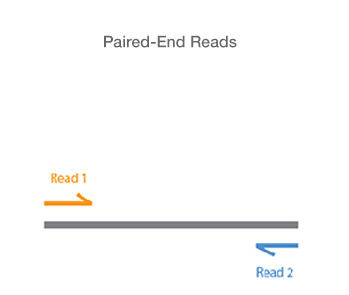
\includegraphics{img/paired_end_reads.png}
\caption{Paired-end Reads}
\end{figure}

    The above image has been taken from
\url{https://www.illumina.com/science/technology/next-generation-sequencing/plan-experiments/read-length.html\#}

    During this process two FASTQ files are produced. One of the FASTQ files
is usually named with \texttt{\_1.fastq} at the end and contains the
sequencing data from `reading' one end of the fragment (reads). The
other FASTQ file is usually named with \texttt{\_2.fastq} at the end and
contains the sequencing data from `reading' the other end of the
fragment (reads). Each fragment has a unique name and the sequence read
for one end of the fragment is labelled with the fragment name followed
by \texttt{/1}. The corresponding sequence read for the other end of the
fragment is labelled with the fragment name followed by \texttt{/2}. The
order in which the reads appear in the FASTQ files is also important as
many tools assume that the first read in the \texttt{\_1.fastq} file and
first read in the \texttt{\_2.fastq} file are from the same fragment and
so on.

    So FASTQ data for an illumina paired end sequencing run might look like:

In one fastq file (e.g.~run\_1.fastq):

\begin{verbatim}
@ERR007731.739 IL16_2979:6:1:9:1684/1
CTTGACGACTTGAAAAATGACGAAATCACTAAAAAACGTGAAAAATGAGAAATG
+
BBCBCBBBBBBBABBABBBBBBBABBBBBBBBBBBBBBABAAAABBBBB=@>B
@ERR007731.740 IL16_2979:6:1:9:1419/1
TAGGGGAAAGTTCTCATGAGTACATCCGAAAAGAGGGCAACCCCAAATCAAAAG
+
BBABBBABABAABABABBABBBAAA>@B@BBAA@4AAA>.>BAA@779:AAA@A
\end{verbatim}

The other fastq file (e.g.~run\_2.fastq):

\begin{verbatim}
@ERR007731.739 IL16_2979:6:1:9:1684/2
GATGACGACCCGAAAAATTACGAAATCACTAGCCAACGTGAATTTTGAGAACTA
+
BBABCBCBBBBBABBABBBBBBBABBBBBBBBBBBBBBAAAAAABBBBBA@>B
@ERR007731.740 IL16_2979:6:1:9:1419/2
AAAAAAAAAGATGTCATCAGCACATCAGAAAAGAAGGCAACTTTAAAACTTTTC
+
BBCBBBABABBABABABBABBBAAA>@BBBBAA@4AAA>.>BAA@779:AA>@A
\end{verbatim}

    \hypertarget{quality-scores}{%
\subsubsection{Quality scores}\label{quality-scores}}

In a FASTQ file, a single character encodes a quality score, typically a
number between 0 and 40 (but in theory this can range between 0-93).
Each character maps to an ASCII value which in turn can be converted to
a quality score.

\begin{longtable}[]{@{}lll@{}}
\toprule
Character & ASCII & FASTQ quality score (ASCII -- 33) \\
\midrule
\endhead
! & 33 & 0 \\
`` & 34 & 1 \\
\# & 35 & 2 \\
\$ & 36 & 3 \\
\% & 37 & 4 \\
\ldots{} & \ldots{} & \ldots{} \\
C & 67 & 34 \\
D & 68 & 35 \\
E & 69 & 36 \\
F & 70 & 37 \\
G & 71 & 38 \\
H & 72 & 39 \\
I & 73 & 40 \\
\bottomrule
\end{longtable}

The first 32 ASCII codes are reserved for characters which are not
printable (e.g.~tab, return, space etc.). None of these can be used in
the quality string, so we subtract 33 from the ASCII value of the
character to determine the quality score. For example, the ASCII code
for ``C'' is 67, so the corresponding quality is:

\begin{verbatim}
Q = 67 - 33 = 34
\end{verbatim}

So, in the FASTQ examples above, most of the base calls have scores in
the 30s, which indicates a high degree of confidence in their accuracy.
A score of 30 denotes a 1 in 1000 chance of an error, i.e.~99.9\%
accuracy.

\begin{longtable}[]{@{}lll@{}}
\toprule
Quality Score & Probability of incorrect base call & Base call
accuracy \\
\midrule
\endhead
10 & 1 in 10 & 90\% \\
20 & 1 in 100 & 99\% \\
30 & 1 in 1000 & 99.9\% \\
40 & 1 in 10,000 & 99.99\% \\
50 & 1 in 100,000 & 99.999\% \\
60 & 1 in 1,000,000 & 99.9999\% \\
\bottomrule
\end{longtable}

You don't need to worry about being able to convert the characters to a
quality score as most of the software tools can interpret them
automatically. But the following perl command will print the quality
score for an ASCII character. Try changing the ``A'' to another
character, for example one from the quality strings above (e.g.~@, = or
B).

    \begin{tcolorbox}[breakable, size=fbox, boxrule=1pt, pad at break*=1mm,colback=cellbackground, colframe=cellborder]
\prompt{In}{incolor}{ }{\boxspacing}
\begin{Verbatim}[commandchars=\\\{\}]
perl\PY{+w}{ }\PYZhy{}e\PY{+w}{ }\PY{l+s+s1}{\PYZsq{}printf \PYZdq{}\PYZpc{}d\PYZbs{}n\PYZdq{},ord(\PYZdq{}A\PYZdq{})\PYZhy{}33;\PYZsq{}}
\end{Verbatim}
\end{tcolorbox}

    \hypertarget{exercises}{%
\subsubsection{Exercises}\label{exercises}}

\textbf{Q2: How many reads are there in the file example.fastq? (Hint:
remember that \texttt{@} is a possible quality score. Is there something
else in the header that is unique?)}

    \begin{tcolorbox}[breakable, size=fbox, boxrule=1pt, pad at break*=1mm,colback=cellbackground, colframe=cellborder]
\prompt{In}{incolor}{ }{\boxspacing}
\begin{Verbatim}[commandchars=\\\{\}]

\end{Verbatim}
\end{tcolorbox}

    Again, don't worry if you cannot solve this, a solution will be provided
during the practical session.

    \textbf{Note}: The FASTQ format is a text based file, however it is
possible (and good practice) to compress these files with \texttt{gzip}.
A gzipped fastq file is usually suffixed with \texttt{.fastq.gz} or
\texttt{.fq.gz}.

    \hypertarget{sambam}{%
\subsection{SAM/BAM}\label{sambam}}

A common task with sequence data is to match or align it to a reference
genome. \href{https://samtools.github.io/hts-specs/SAMv1.pdf}{SAM
(Sequence Alignment/Map)} is a standard format for storing sequence read
alignments to a reference genome. If no reference genome is available,
the data can be stored unaligned. SAM is a text based file. BAM is the
compressed binary version of SAM. Compressed binary files are not
readable by a human but are smaller than the corresponding uncompressed
file meaning they take up less disk space and make it easier and quicker
to copy files between locations.

SAM/BAM files consist of a header section (optional) and an alignment
section. The alignment section contains one record (a fragment
alignment) per line describing the alignment between fragment and
reference. Each record has 11 fixed columns and optional key:type:value
tuples. Open the
\href{https://samtools.github.io/hts-specs/SAMv1.pdf}{SAM/BAM file
specification document} as you may need to refer to it throughout this
tutorial.

Now let us have a closer look at the different parts of the SAM/BAM
files.

\hypertarget{header-section}{%
\subsubsection{Header Section}\label{header-section}}

Each line or record in the SAM header starts with an \texttt{@},
followed by a two-letter code defining the record type (the different
types are defined in the
\href{https://samtools.github.io/hts-specs/SAMv1.pdf}{SAM/BAM format
specification document}). Each line or record contains meta-data for
that specific record which is captured as a series of key-value pairs in
the format of `TAG:VALUE'.

\hypertarget{read-groups}{%
\paragraph{Read groups}\label{read-groups}}

One useful record type is RG which can be used to describe each unit of
sequencing, e.g.~a barcode or lane of sequencing data for Illumina. The
RG code can be used to capture extra meta-data for the unit of
sequencing. Some common RG TAGs are:

\begin{itemize}
\tightlist
\item
  ID: Read group identifier
\item
  PL: Sequencing platform
\item
  LB: Library name
\item
  PI: Predicted insert/fragment size
\item
  DS: Description
\item
  SM: Sample identifier
\item
  CN: Sequencing centre
\end{itemize}

    \hypertarget{exercises}{%
\subsubsection{Exercises}\label{exercises}}

Look at the following line from the header of the SAM/BAM file and
answer the questions that follow:

\begin{verbatim}
@RG ID:ERR003612 PL:ILLUMINA LB:g1k-sc-NA20538-TOS-1 PI:2000 DS:SRP000540 SM:NA20538 CN:SC
\end{verbatim}

You may want to refer to section 1.3 of the SAM specification.

\textbf{Q3: What does RG stand for?}

    \begin{tcolorbox}[breakable, size=fbox, boxrule=1pt, pad at break*=1mm,colback=cellbackground, colframe=cellborder]
\prompt{In}{incolor}{ }{\boxspacing}
\begin{Verbatim}[commandchars=\\\{\}]

\end{Verbatim}
\end{tcolorbox}

    \textbf{Q4: What platform was used to produce the data?}

    \begin{tcolorbox}[breakable, size=fbox, boxrule=1pt, pad at break*=1mm,colback=cellbackground, colframe=cellborder]
\prompt{In}{incolor}{ }{\boxspacing}
\begin{Verbatim}[commandchars=\\\{\}]

\end{Verbatim}
\end{tcolorbox}

    \textbf{Q5: Where was the sequence data produced?}

    \begin{tcolorbox}[breakable, size=fbox, boxrule=1pt, pad at break*=1mm,colback=cellbackground, colframe=cellborder]
\prompt{In}{incolor}{ }{\boxspacing}
\begin{Verbatim}[commandchars=\\\{\}]

\end{Verbatim}
\end{tcolorbox}

    \textbf{Q6: What is the expected insert/fragment size?}

    \begin{tcolorbox}[breakable, size=fbox, boxrule=1pt, pad at break*=1mm,colback=cellbackground, colframe=cellborder]
\prompt{In}{incolor}{ }{\boxspacing}
\begin{Verbatim}[commandchars=\\\{\}]

\end{Verbatim}
\end{tcolorbox}

    \hypertarget{alignment-section}{%
\subsubsection{Alignment Section}\label{alignment-section}}

The alignment section of a SAM file contains one line per alignment.
Each line consists of 12 fields/columns described below. The first 11
columns are mandatory.

\begin{enumerate}
\def\labelenumi{\arabic{enumi}.}
\tightlist
\item
  QNAME: Query NAME of the read or the read pair
\item
  FLAG: Bitwise FLAG (pairing, strand, mate strand, etc.)
\item
  RNAME: Reference sequence NAME
\item
  POS: 1-Based leftmost POSition of clipped alignment
\item
  MAPQ: MAPping Quality (Phred-scaled)
\item
  CIGAR: Extended CIGAR string (operations: MIDNSHPX=)
\item
  MRNM: Mate Reference NaMe ('=' if same as RNAME)
\item
  MPOS: 1-Based leftmost Mate POSition
\item
  ISIZE: Inferred Insert SIZE
\item
  SEQ: Query SEQuence on the same strand as the reference
\item
  QUAL: Query QUALity (ASCII-33=Phred base quality)
\item
  OTHER: Optional fields
\end{enumerate}

The image below provides a visual guide to some of the fields/columns of
the SAM format.

    \begin{figure}
\centering
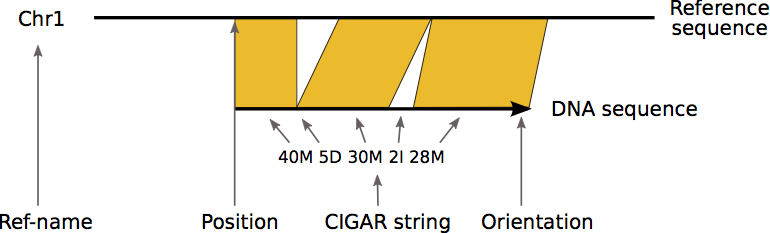
\includegraphics{img/SAM_BAM.png}
\caption{SAM format}
\end{figure}

    In a SAM file, the alignment in this image would be represented in a
SAM/BAM file as:

\texttt{fragment001\ \ \ \ 163\ Chr1\ \ \ \ 19999970\ \ \ \ 23\ \ 40M5D30M2I28M\ \ \ =\ \ \ 20000147\ \ \ \ 213\ GGTGCGTGGAT...\ \ \ \ \textless{}=@A@??@=A...}

\hypertarget{exercises}{%
\subsubsection{Exercises}\label{exercises}}

Let's have a look at example.sam. Notice that we can use the standard
Linux operations like \textbf{less} on this file.

    \begin{tcolorbox}[breakable, size=fbox, boxrule=1pt, pad at break*=1mm,colback=cellbackground, colframe=cellborder]
\prompt{In}{incolor}{ }{\boxspacing}
\begin{Verbatim}[commandchars=\\\{\}]
less\PY{+w}{ }\PYZhy{}S\PY{+w}{ }example.sam
\end{Verbatim}
\end{tcolorbox}

    \textbf{Q7: What is the mapping quality of ERR003762.5016205? (Hint: can
you use grep and awk to find this?)}

    \begin{tcolorbox}[breakable, size=fbox, boxrule=1pt, pad at break*=1mm,colback=cellbackground, colframe=cellborder]
\prompt{In}{incolor}{ }{\boxspacing}
\begin{Verbatim}[commandchars=\\\{\}]

\end{Verbatim}
\end{tcolorbox}

    \textbf{Q8: What is the CIGAR string for ERR003814.6979522? (We will go
through the meaning of CIGAR strings in the next section)}

    \begin{tcolorbox}[breakable, size=fbox, boxrule=1pt, pad at break*=1mm,colback=cellbackground, colframe=cellborder]
\prompt{In}{incolor}{ }{\boxspacing}
\begin{Verbatim}[commandchars=\\\{\}]

\end{Verbatim}
\end{tcolorbox}

    \textbf{Q9: What is the inferred insert/fragment size for
ERR003814.1408899?}

    \begin{tcolorbox}[breakable, size=fbox, boxrule=1pt, pad at break*=1mm,colback=cellbackground, colframe=cellborder]
\prompt{In}{incolor}{ }{\boxspacing}
\begin{Verbatim}[commandchars=\\\{\}]

\end{Verbatim}
\end{tcolorbox}

    \hypertarget{cigar-string}{%
\subsubsection{CIGAR string}\label{cigar-string}}

Column 6 of the alignment is the CIGAR string for that alignment. The
CIGAR string provides a compact representation of sequence alignment.
Have a look at the table below. It contains the meaning of all different
symbols of a CIGAR string:

\begin{longtable}[]{@{}ll@{}}
\toprule
Symbol & Meaning \\
\midrule
\endhead
M & alignment match or mismatch \\
= & sequence match \\
X & sequence mismatch \\
I & insertion into the reference \\
D & deletion from the reference \\
S & soft clipping (clipped sequences present in SEQ) \\
H & hard clipping (clipped sequences NOT present in SEQ) \\
N & skipped region from the reference \\
P & padding (silent deletion from padded reference) \\
\bottomrule
\end{longtable}

Below are two examples describing the CIGAR string in more detail.

\textbf{Example 1:}\\
Ref:~~~~~ACGTACGTACGTACGT\\
Read:~~ACGT-~-~-~-~ACGTACGA\\
Cigar: 4M 4D 8M

The first four bases in the read are the same as in the reference, so we
can represent these as 4M in the CIGAR string. Next is a deletion of 4
bases, represented by 4D, followed by 7 alignment matches and one
alignment mismatch, represented by 8M. Note that the mismatch at
position 16 is included in 8M. This is because it still aligns to the
reference.

\textbf{Example 2:}\\
Ref:~~~~~ACTCAGTG-~-~GT\\
Read:~~ACGCA-~TGCAGTtagacgt\\
Cigar: 5M 1D 2M 2I 2M 7S

Here we start with 5 alignment matches and mismatches, followed by a
deletion of one base. Then we have two more alignment matches, an
insertion of 2 bases and two more matches. At the end, we have a soft
clipping of 7 bases, 7S. These are clipped sequences that are present in
the read but do not match the reference.

\hypertarget{exercises}{%
\subsubsection{Exercises}\label{exercises}}

\textbf{Q10: What does the CIGAR from Q8 mean?}

    \begin{tcolorbox}[breakable, size=fbox, boxrule=1pt, pad at break*=1mm,colback=cellbackground, colframe=cellborder]
\prompt{In}{incolor}{ }{\boxspacing}
\begin{Verbatim}[commandchars=\\\{\}]

\end{Verbatim}
\end{tcolorbox}

    \textbf{Q11: How would you represent the following alignment with a
CIGAR string?}

Ref:~~~~~ACGT-~-~-~-~ACGTACGT\\
Read:~~ACGTACGTACGTACGT

    \begin{tcolorbox}[breakable, size=fbox, boxrule=1pt, pad at break*=1mm,colback=cellbackground, colframe=cellborder]
\prompt{In}{incolor}{ }{\boxspacing}
\begin{Verbatim}[commandchars=\\\{\}]

\end{Verbatim}
\end{tcolorbox}

    \hypertarget{flags}{%
\subsubsection{Flags}\label{flags}}

Column 2 of the alignment contains a combination of bitwise FLAGs
providing detailed information about the alignment. The following table
details the meaning of each flag

\begin{longtable}[]{@{}llll@{}}
\toprule
Hex & Dec & Flag & Description \\
\midrule
\endhead
0x1 & 1 & PAIRED & paired-end (or multiple-segment) sequencing
technology \\
0x2 & 2 & PROPER\_PAIR & each segment properly aligned according to the
aligner \\
0x4 & 4 & UNMAP & segment unmapped \\
0x8 & 8 & MUNMAP & next segment in the template unmapped \\
0x10 & 16 & REVERSE & SEQ is reverse complemented \\
0x20 & 32 & MREVERSE & SEQ of the next segment in the template is
reversed \\
0x40 & 64 & READ1 & the first segment in the template \\
0x80 & 128 & READ2 & the last segment in the template \\
0x100 & 256 & SECONDARY & secondary alignment \\
0x200 & 512 & QCFAIL & not passing quality controls \\
0x400 & 1024 & DUP & PCR or optical duplicate \\
0x800 & 2048 & SUPPLEMENTARY & supplementary alignment \\
\bottomrule
\end{longtable}

For example, if you have an alignment with FLAG set to 113, this can
only be represented by decimal numbers \texttt{64\ +\ 32\ +\ 16\ +\ 1},
so we know that these four flags apply to the alignment and the
alignment is paired, reverse complemented, the sequence of the next
template/read in the fragment is reversed and the read aligned is the
first read in the template.

\hypertarget{primary-secondary-and-supplementary-alignments}{%
\paragraph{Primary, secondary and supplementary
alignments}\label{primary-secondary-and-supplementary-alignments}}

A read that aligns to a single position in a reference (including
insertions, deletions, skips and clipping but not direction changes), is
a \textbf{linear alignment}. If a read cannot be represented as a linear
alignment, but instead is represented as a group of linear alignments
without large overlaps, it is called a \textbf{chimeric alignment}.
These can for instance be caused by structural variations. Usually, one
of the linear alignments in a chimeric alignment is considered to be the
\textbf{representative} alignment, and the others are called
\textbf{supplementary}.

Sometimes a read maps equally well to more than one location. In these
cases, one of the possible alignments is marked as the \textbf{primary}
alignment and the rest are marked as \textbf{secondary} alignments.

\hypertarget{bam}{%
\subsubsection{BAM}\label{bam}}

BAM (Binary Alignment/Map) format, is a binary compressed version of
SAM. This means that, while SAM is human readable, BAM is only readable
for computers. BAM files can be viewed using samtools, and will then
have the same format as a SAM file. The key features of BAM are:

\begin{itemize}
\tightlist
\item
  Stores alignments from most mapping tools
\item
  Supports multiple sequencing technologies
\item
  Supports indexing for quick retrieval/viewing of alignments
\item
  Compact size (e.g.~112Gbp Illumina = 116GB disk space)
\item
  Reads can be grouped into logical groups e.g.~lanes, libraries,
  samples
\item
  Widely supported by variant calling packages and genome viewers
\end{itemize}

    \hypertarget{exercises}{%
\subsubsection{Exercises}\label{exercises}}

Since BAM is a binary format, we can't use the standard Linux operations
(cat, less, head, grep etc.) directly on this format. \texttt{Samtools}
is a set of programs for interacting with SAM and BAM files. Using the
\textbf{samtools view} command, print the header of the BAM file:

    \begin{tcolorbox}[breakable, size=fbox, boxrule=1pt, pad at break*=1mm,colback=cellbackground, colframe=cellborder]
\prompt{In}{incolor}{ }{\boxspacing}
\begin{Verbatim}[commandchars=\\\{\}]
samtools\PY{+w}{ }view\PY{+w}{ }\PYZhy{}H\PY{+w}{ }NA20538.bam
\end{Verbatim}
\end{tcolorbox}

    \textbf{Q12: What version of the human assembly was used to perform the
alignments? (Hint: Can you spot this somewhere in the @SQ records?)}

    \begin{tcolorbox}[breakable, size=fbox, boxrule=1pt, pad at break*=1mm,colback=cellbackground, colframe=cellborder]
\prompt{In}{incolor}{ }{\boxspacing}
\begin{Verbatim}[commandchars=\\\{\}]

\end{Verbatim}
\end{tcolorbox}

    \textbf{Q13: How many sequencing runs/lanes are in this BAM file? (Hint:
Do you recall what RG represents?)}

    \begin{tcolorbox}[breakable, size=fbox, boxrule=1pt, pad at break*=1mm,colback=cellbackground, colframe=cellborder]
\prompt{In}{incolor}{ }{\boxspacing}
\begin{Verbatim}[commandchars=\\\{\}]

\end{Verbatim}
\end{tcolorbox}

    \textbf{Q14: What programs were used to create this BAM file? (Hint:
have a look for the program record, @PG)}

    \begin{tcolorbox}[breakable, size=fbox, boxrule=1pt, pad at break*=1mm,colback=cellbackground, colframe=cellborder]
\prompt{In}{incolor}{ }{\boxspacing}
\begin{Verbatim}[commandchars=\\\{\}]

\end{Verbatim}
\end{tcolorbox}

    \textbf{Q15: What version of bwa was used to align the reads? (Hint: is
there anything in the @PG record that looks like it could be a version
tag?)}

    \begin{tcolorbox}[breakable, size=fbox, boxrule=1pt, pad at break*=1mm,colback=cellbackground, colframe=cellborder]
\prompt{In}{incolor}{ }{\boxspacing}
\begin{Verbatim}[commandchars=\\\{\}]

\end{Verbatim}
\end{tcolorbox}

    Running \textbf{samtools view} on a BAM file without any options will
produce SAM format without the header information. This is printed to
the STDOUT in the terminal (screen). Let's have a look at the first read
of the BAM file:

    \begin{tcolorbox}[breakable, size=fbox, boxrule=1pt, pad at break*=1mm,colback=cellbackground, colframe=cellborder]
\prompt{In}{incolor}{ }{\boxspacing}
\begin{Verbatim}[commandchars=\\\{\}]
samtools\PY{+w}{ }view\PY{+w}{ }NA20538.bam\PY{+w}{ }\PY{p}{|}\PY{+w}{ }head\PY{+w}{ }\PYZhy{}n\PY{+w}{ }\PY{l+m}{1}
\end{Verbatim}
\end{tcolorbox}

    Note we only want to look at the first line of the alignment section of
the BAM file so we have piped the output of \texttt{samtools\ view} to
the \texttt{head} command.

    \textbf{Q16: What is the name of the first read? (Hint: have a look at
the \href{formats.ipynb\#Alignment-Section}{alignment section} if you
can't recall the different fields)}

    \begin{tcolorbox}[breakable, size=fbox, boxrule=1pt, pad at break*=1mm,colback=cellbackground, colframe=cellborder]
\prompt{In}{incolor}{ }{\boxspacing}
\begin{Verbatim}[commandchars=\\\{\}]

\end{Verbatim}
\end{tcolorbox}

    \textbf{Q17: What position does the alignment start at?}

    \begin{tcolorbox}[breakable, size=fbox, boxrule=1pt, pad at break*=1mm,colback=cellbackground, colframe=cellborder]
\prompt{In}{incolor}{ }{\boxspacing}
\begin{Verbatim}[commandchars=\\\{\}]

\end{Verbatim}
\end{tcolorbox}

    \hypertarget{cram}{%
\subsection{CRAM}\label{cram}}

Even though BAM files are compressed, they are still very large.
Typically they use 1.5-2 bytes for each base pair of sequencing data
that they contain, and while disk capacity is ever improving, increases
in disk capacity are being far outstripped by sequencing technologies.

    \begin{figure}
\centering
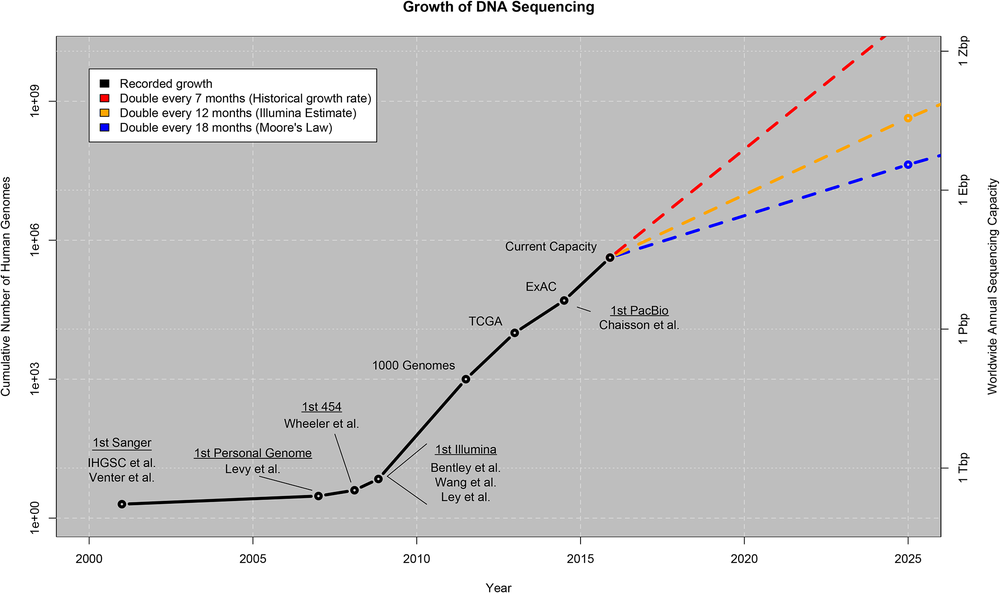
\includegraphics{img/compression_cram.png}
\caption{Growth of DNA sequencing}
\end{figure}

    BAM stores all the data for a sequence read, this includes every base
call and every base quality, and it uses a single compression technique
for all types of data (numbers, characters etc.). Therefore, CRAM was
designed to provide a way to store the same information as BAM but using
less disk space. CRAM uses three important concepts:

\begin{itemize}
\tightlist
\item
  Reference based compression
\item
  Controlled loss of quality information
\item
  Different compression methods to suit the type of data, e.g.~base
  qualities vs.~metadata vs.~extra tags
\end{itemize}

The figure below displays how reference-based compression works. Instead
of storing all the bases of all the reads, only the nucleotides that
differ from the reference, and their positions, are kept.

    \begin{figure}
\centering
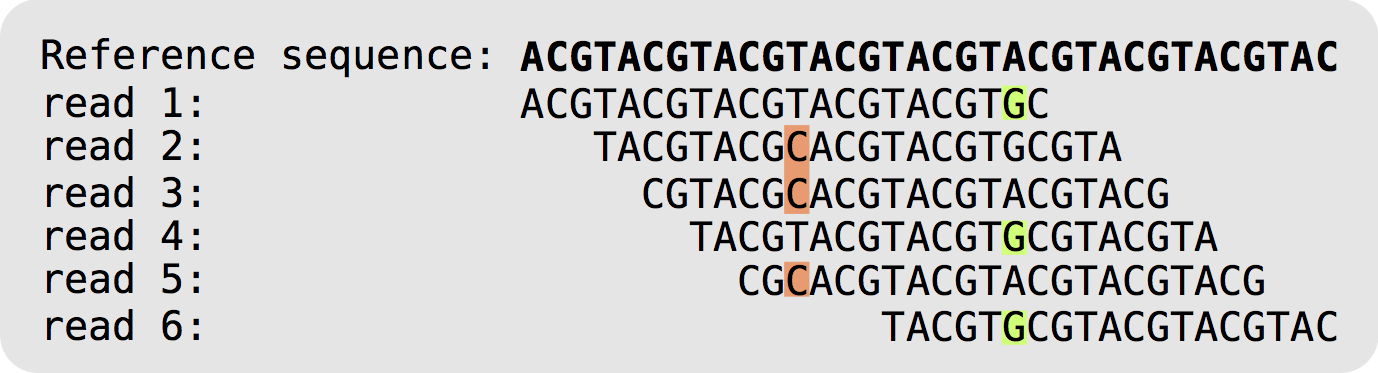
\includegraphics{img/CRAM_format.png}
\caption{CRAM1}
\end{figure}

    \begin{figure}
\centering
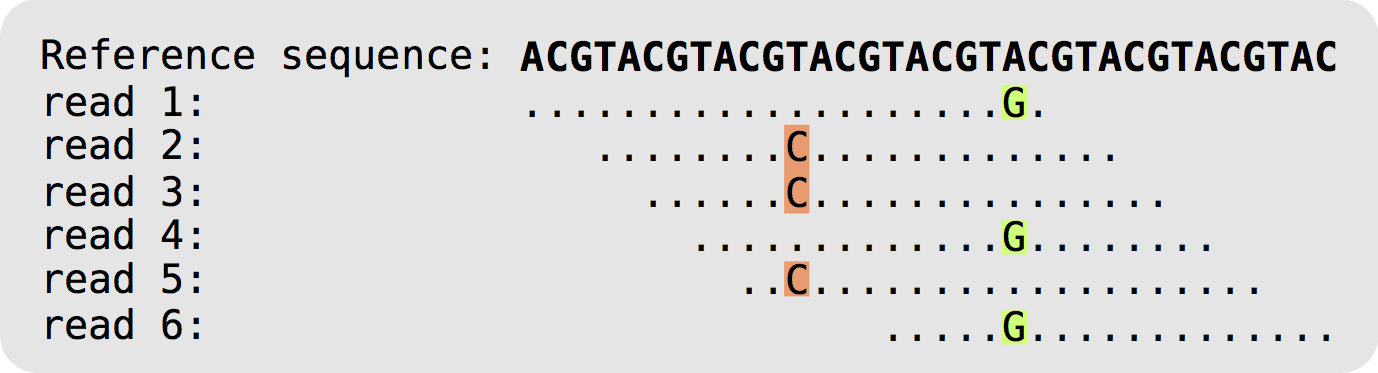
\includegraphics{img/CRAM_format2.png}
\caption{CRAM2}
\end{figure}

    This means that the same information from a BAM file can be stored in
CRAM file but using a fraction of the disk space.

    \hypertarget{sorting-and-indexing}{%
\subsection{Sorting and Indexing}\label{sorting-and-indexing}}

The reads in a BAM and CRAM file can be ordered or sorted in one of two
ways:

\begin{itemize}
\tightlist
\item
  sorted by name, meaning the reads are ordered based on the fragment
  name so reads from the same fragment (read pairs) will appear next to
  each other in the file
\item
  coordinate-sorted, meaning the reads that align to the leftmost
  position or start of the genome appear first in the file.
\end{itemize}

To allow for fast random access of regions in BAM and CRAM files, they
can be indexed. The files must first be coordinate-sorted. This can be
done using \textbf{samtools sort}. If no options are supplied, it will
by default sort by the left-most position.

    \begin{tcolorbox}[breakable, size=fbox, boxrule=1pt, pad at break*=1mm,colback=cellbackground, colframe=cellborder]
\prompt{In}{incolor}{ }{\boxspacing}
\begin{Verbatim}[commandchars=\\\{\}]
samtools\PY{+w}{ }sort\PY{+w}{ }\PYZhy{}o\PY{+w}{ }NA20538\PYZus{}sorted.bam\PY{+w}{ }NA20538.bam
\end{Verbatim}
\end{tcolorbox}

    Now we can use \textbf{samtools index} to create an index file (.bai)
for our sorted BAM file:

    \begin{tcolorbox}[breakable, size=fbox, boxrule=1pt, pad at break*=1mm,colback=cellbackground, colframe=cellborder]
\prompt{In}{incolor}{ }{\boxspacing}
\begin{Verbatim}[commandchars=\\\{\}]
samtools\PY{+w}{ }index\PY{+w}{ }NA20538\PYZus{}sorted.bam
\end{Verbatim}
\end{tcolorbox}

    You can think on an index file as a lookup table that tools like
samtools can use to easily and quickly retrive a segment of the file
without having to read the entire file into memory. For example, to look
for reads mapped to a specific region, we can use \textbf{samtools view}
and specify the region we are interested in as:
RNAME{[}:STARTPOS{[}-ENDPOS{]}{]}.

    If we wanted to look at all the reads mapped to chromosome 1, we could
use:

    \begin{tcolorbox}[breakable, size=fbox, boxrule=1pt, pad at break*=1mm,colback=cellbackground, colframe=cellborder]
\prompt{In}{incolor}{ }{\boxspacing}
\begin{Verbatim}[commandchars=\\\{\}]
samtools\PY{+w}{ }view\PY{+w}{ }NA20538\PYZus{}sorted.bam\PY{+w}{ }\PY{l+m}{1}\PY{+w}{ }\PY{p}{|}\PY{+w}{ }head\PY{+w}{ }\PYZhy{}10
\end{Verbatim}
\end{tcolorbox}

    To look at the region on chromosome 1 beginning at position 25,000,000
and ending at the end of the chromosome, we can do:

    \begin{tcolorbox}[breakable, size=fbox, boxrule=1pt, pad at break*=1mm,colback=cellbackground, colframe=cellborder]
\prompt{In}{incolor}{ }{\boxspacing}
\begin{Verbatim}[commandchars=\\\{\}]
samtools\PY{+w}{ }view\PY{+w}{ }NA20538\PYZus{}sorted.bam\PY{+w}{ }\PY{l+m}{1}:25000000
\end{Verbatim}
\end{tcolorbox}

    And to explore the 1001bp long region on chromosome 1 beginning at
position 20,000,000 and ending at position 20,001,000, we can use:

    \begin{tcolorbox}[breakable, size=fbox, boxrule=1pt, pad at break*=1mm,colback=cellbackground, colframe=cellborder]
\prompt{In}{incolor}{ }{\boxspacing}
\begin{Verbatim}[commandchars=\\\{\}]
samtools\PY{+w}{ }view\PY{+w}{ }NA20538\PYZus{}sorted.bam\PY{+w}{ }\PY{l+m}{1}:20000000\PYZhy{}20001000\PY{+w}{ }\PY{p}{|}\PY{+w}{ }tail\PY{+w}{ }\PYZhy{}10
\end{Verbatim}
\end{tcolorbox}

    \hypertarget{exercises}{%
\subsubsection{Exercises}\label{exercises}}

\textbf{Q18: How many reads are mapped to region 20025000-20030000 on
chromosome 1?}

    \begin{tcolorbox}[breakable, size=fbox, boxrule=1pt, pad at break*=1mm,colback=cellbackground, colframe=cellborder]
\prompt{In}{incolor}{ }{\boxspacing}
\begin{Verbatim}[commandchars=\\\{\}]

\end{Verbatim}
\end{tcolorbox}

    \hypertarget{vcfbcf}{%
\subsection{VCF/BCF}\label{vcfbcf}}

The VCF format is a standard format for storing sequence variation data.
The BCF format is the compressed binary version of VCF. Remember that a
compressed binary file is not human readable.

VCF is a text based tab-delimited file that is parsable by standard
Linux commands. It is composed of two parts, the VCF header and the
body. The figure below provides an overview of the different components
of a VCF file:

    \begin{figure}
\centering
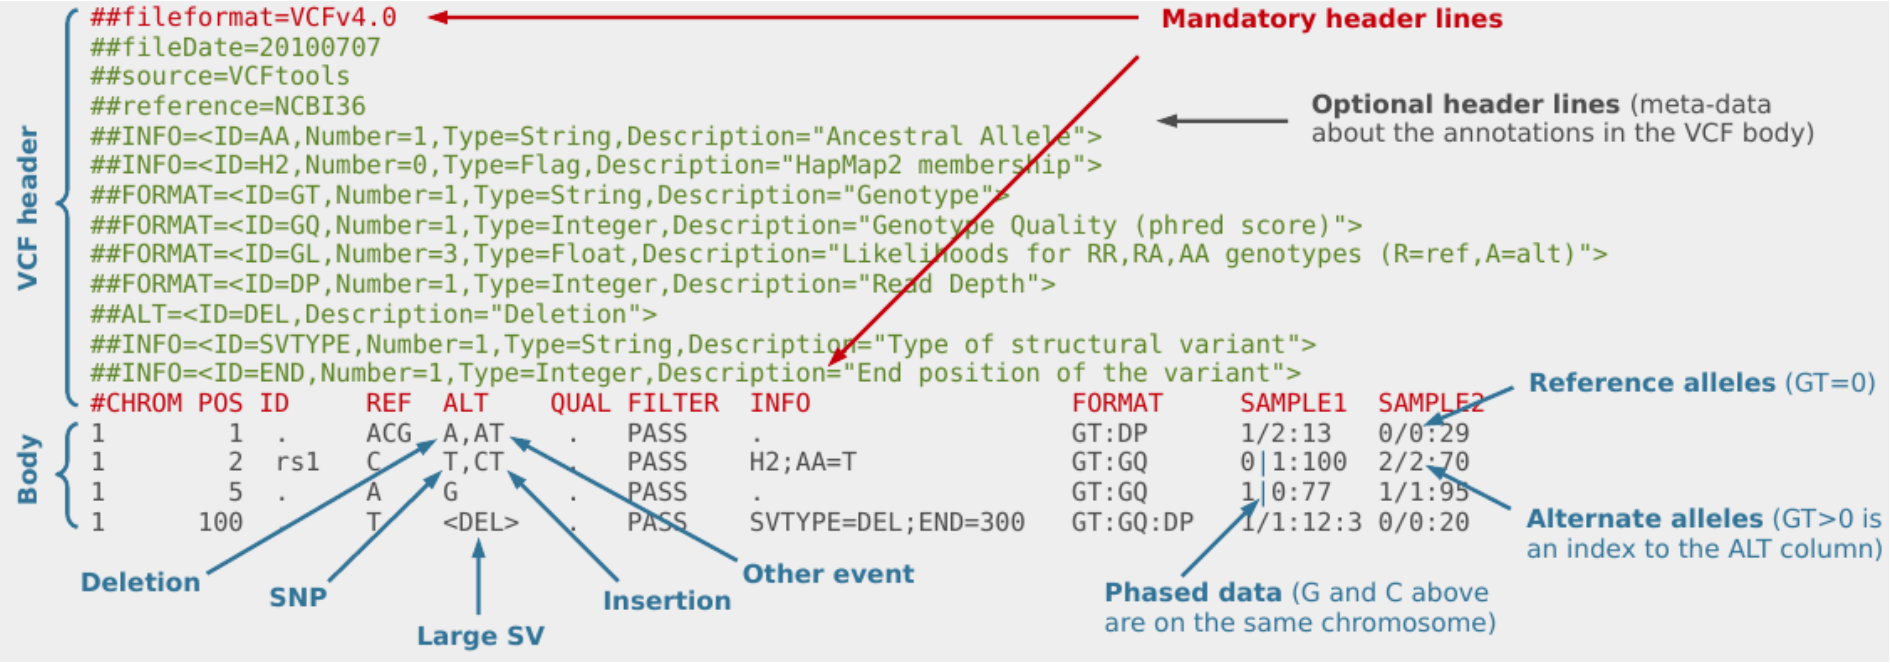
\includegraphics{img/VCF1.png}
\caption{VCF format}
\end{figure}

    \hypertarget{vcf-header}{%
\subsubsection{VCF header}\label{vcf-header}}

Header lines are denoted with \texttt{\#\#} and provide metadata about
the file (e.g.~fileformat, fileDate and reference) and metadata defining
the fields used in the body of the file (e.g.~INFO, FILTER, and FORMAT).
These header lines consist of key=value pairs and can consist of
multiple pairs enclosed by \texttt{\textless{}\textgreater{}}. More
information about these fields is available in the
\href{http://samtools.github.io/hts-specs/VCFv4.3.pdf}{VCF
specification}.

All header lines are optional and can be put in any order, except for
\textit{fileformat}. This holds the information about which version of VCF
is used and must come first in the file.

\hypertarget{vcf-body}{%
\subsubsection{VCF body}\label{vcf-body}}

The body of the VCF follows the header, and is tab separated into 8
mandatory columns and an unlimited number of optional columns that may
be used to record other information about the sample(s).

\hypertarget{header-line}{%
\paragraph{Header line}\label{header-line}}

The header line starts with \texttt{\#} and contains the names of the
columns used in the file:

\begin{enumerate}
\def\labelenumi{\arabic{enumi}.}
\tightlist
\item
  CHROM: an identifier from the reference genome
\item
  POS: the reference position
\item
  ID: a list of unique identifiers (where available)
\item
  REF: the reference base(s)
\item
  ALT: the alternate base(s)
\item
  QUAL: a phred-scaled quality score
\item
  FILTER: filter status
\item
  INFO: additional information
\end{enumerate}

If the file contains genotype data, additional fields are included in
the file. These are a FORMAT column, and then a number of sample IDs.
The FORMAT field defines the data types and order of the information for
each sample. Some examples of these data types are:

\begin{itemize}
\tightlist
\item
  GT: Genotype, encoded as allele values separated by either of / or
  \textbar{}
\item
  DP: Read depth at this position for this sample
\item
  GQ: Conditional genotype quality, encoded as a phred quality
\end{itemize}

\hypertarget{positions}{%
\paragraph{Positions}\label{positions}}

Following the header line is a series of rows containing information
about a position in the genome along with genotype information at that
position for each of the samples.

Let's look at a specific example:

    \begin{figure}
\centering

\includegraphics{img/vcf_example.png}
\caption{VCF Example Line}
\end{figure}

    The locations is position 3 on chromosome 1, the variant site does not
have an identifier in a standard database. The reference base is an A at
this position and all the alternative alleles called in all samples is
G. There is no quality score for the site and it passes the quality
filters that have been applied. The vallues for AC,AN and DP for this
site across all samples is AC=67, AN=5400, DP=2809. The definition of
AC, AN and DP can be found in the INFO lines in the header of the VCF
and AC is allele count, AN is allele number and DP is read depth. The
remainder of the columns provide information about the site in each
sample. First the FORMAT column describes the information listed for
each sample, GT, PL, DP, GQ. Again the definition of these will be found
in the VCF header and are defined as genotype, genotype liklihoods, read
depth and genotype quality. This means for SAMPLE1 the geneotype is 1/1
(G/G), the genotype liklihoods are 0,9,73, the depth at this position in
this sample is 26 and the genotype quality is 22. Similarily for SAMPLE2
the geneotype is 0/0 (A/A), the genotype liklihoods are 0,9,73, the
depth at this position in this sample is 13 and the genotype quality is
22.

    \hypertarget{bcf}{%
\subsubsection{BCF}\label{bcf}}

VCF files can be compressed (for example with gzip), but even compressed
they can still be very large. For example, a compressed VCF with 3781
samples of human data will be 54 GB for chromosome 1, and 680 GB for the
whole genome.

VCFs can also be slow to parse, as text conversion is slow. The main
bottleneck is the ``FORMAT'' fields. For this reason the BCF format, a
binary representation of VCF, was developed. In BCF files the fields are
rearranged for better compresion and fast access. The following images
show the process of converting a VCF file into a BCF file.

    \begin{figure}
\centering
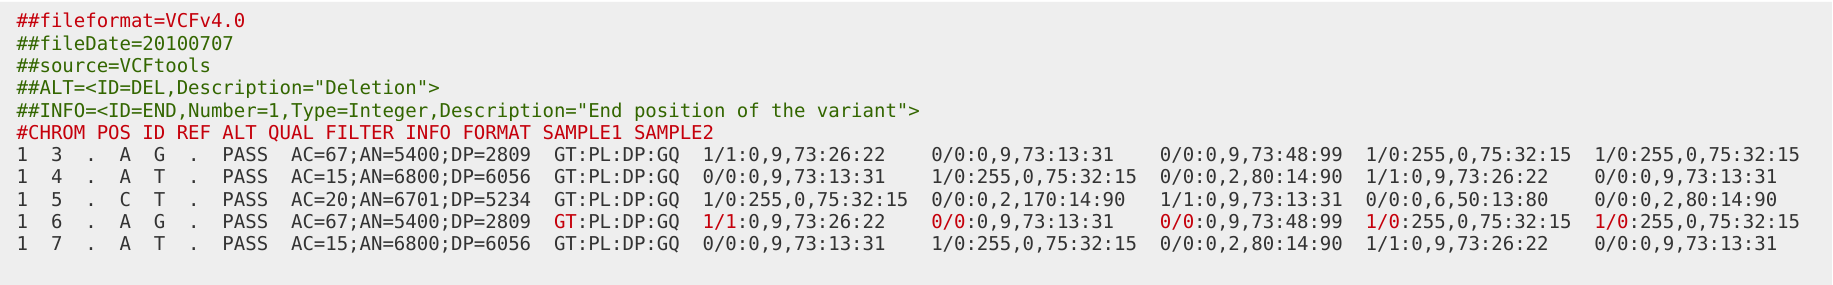
\includegraphics{img/VCF2.png}
\caption{VCF2}
\end{figure}

    \begin{figure}
\centering
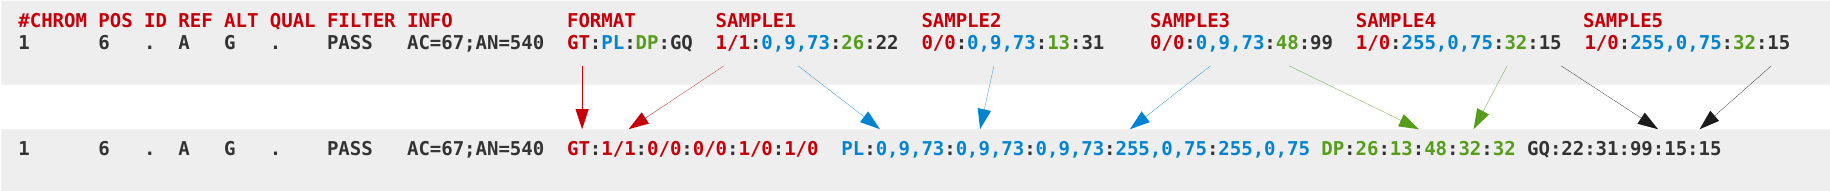
\includegraphics{img/VCF3.png}
\caption{VCF3}
\end{figure}

    \texttt{Bcftools} comprises a set of programs for interacting with VCF
and BCF files. It can be used to view or extract records from a region
and to convert between VCF and BCF formats.

\hypertarget{bcftools-view}{%
\paragraph{bcftools view}\label{bcftools-view}}

Let's have a look at the header of the file 1kg.bcf in the data
directory. Note that \texttt{bcftools} uses \textbf{\texttt{-h}} to
print only the header, while samtools uses \textbf{\texttt{-H}} for
this.

    \begin{tcolorbox}[breakable, size=fbox, boxrule=1pt, pad at break*=1mm,colback=cellbackground, colframe=cellborder]
\prompt{In}{incolor}{ }{\boxspacing}
\begin{Verbatim}[commandchars=\\\{\}]
bcftools\PY{+w}{ }view\PY{+w}{ }\PYZhy{}h\PY{+w}{ }1kg.bcf
\end{Verbatim}
\end{tcolorbox}

    Similarly to BAM, BCF supports random access, that is, fast retrieval
from a given region. For this, the file must be indexed:

    \begin{tcolorbox}[breakable, size=fbox, boxrule=1pt, pad at break*=1mm,colback=cellbackground, colframe=cellborder]
\prompt{In}{incolor}{ }{\boxspacing}
\begin{Verbatim}[commandchars=\\\{\}]
bcftools\PY{+w}{ }index\PY{+w}{ }1kg.bcf
\end{Verbatim}
\end{tcolorbox}

    Now we can extract all records from the region 20:24042765-24043073,
using the \textbf{\texttt{-r}} option. The \textbf{\texttt{-H}} option
will make sure we don't include the header in the output:

    \begin{tcolorbox}[breakable, size=fbox, boxrule=1pt, pad at break*=1mm,colback=cellbackground, colframe=cellborder]
\prompt{In}{incolor}{ }{\boxspacing}
\begin{Verbatim}[commandchars=\\\{\}]
bcftools\PY{+w}{ }view\PY{+w}{ }\PYZhy{}H\PY{+w}{ }\PYZhy{}r\PY{+w}{ }\PY{l+m}{20}:24042765\PYZhy{}24043073\PY{+w}{ }1kg.bcf
\end{Verbatim}
\end{tcolorbox}

    \hypertarget{bcftools-query}{%
\paragraph{bcftools query}\label{bcftools-query}}

The versatile \textbf{bcftools query} command can be used to extract any
VCF field. Combined with standard Linux commands, this gives a powerful
tool for quick querying of VCFs. Have a look at the usage options:

    \begin{tcolorbox}[breakable, size=fbox, boxrule=1pt, pad at break*=1mm,colback=cellbackground, colframe=cellborder]
\prompt{In}{incolor}{ }{\boxspacing}
\begin{Verbatim}[commandchars=\\\{\}]
bcftools\PY{+w}{ }query\PY{+w}{ }\PYZhy{}h
\end{Verbatim}
\end{tcolorbox}

    Let's try out some useful options. As you can see from the usage,
\textbf{\texttt{-l}} will print a list of all the samples in the file.
Give this a go:

    \begin{tcolorbox}[breakable, size=fbox, boxrule=1pt, pad at break*=1mm,colback=cellbackground, colframe=cellborder]
\prompt{In}{incolor}{ }{\boxspacing}
\begin{Verbatim}[commandchars=\\\{\}]
bcftools\PY{+w}{ }query\PY{+w}{ }\PYZhy{}l\PY{+w}{ }1kg.bcf
\end{Verbatim}
\end{tcolorbox}

    Another useful option is \textbf{\texttt{-s}} which allows you to
extract all the data relating to a particular sample. Try this for
sample HG00131:

    \begin{tcolorbox}[breakable, size=fbox, boxrule=1pt, pad at break*=1mm,colback=cellbackground, colframe=cellborder]
\prompt{In}{incolor}{ }{\boxspacing}
\begin{Verbatim}[commandchars=\\\{\}]
bcftools\PY{+w}{ }view\PY{+w}{ }\PYZhy{}s\PY{+w}{ }HG00131\PY{+w}{ }1kg.bcf\PY{+w}{ }\PY{p}{|}\PY{+w}{ }head\PY{+w}{ }\PYZhy{}n\PY{+w}{ }\PY{l+m}{50}
\end{Verbatim}
\end{tcolorbox}

    The format option, \textbf{\texttt{-f}} can be used to select what gets
printed from your query command. For example, the following will print
the position, reference base and alternate base for sample HG00131,
separated by tabs:

    \begin{tcolorbox}[breakable, size=fbox, boxrule=1pt, pad at break*=1mm,colback=cellbackground, colframe=cellborder]
\prompt{In}{incolor}{ }{\boxspacing}
\begin{Verbatim}[commandchars=\\\{\}]
bcftools\PY{+w}{ }query\PY{+w}{ }\PYZhy{}f\PY{l+s+s1}{\PYZsq{}\PYZpc{}POS\PYZbs{}t\PYZpc{}REF\PYZbs{}t\PYZpc{}ALT\PYZbs{}n\PYZsq{}}\PY{+w}{ }\PYZhy{}s\PY{+w}{ }HG00131\PY{+w}{ }1kg.bcf\PY{+w}{ }\PY{p}{|}\PY{+w}{ }head
\end{Verbatim}
\end{tcolorbox}

    \hypertarget{exercises}{%
\subsubsection{Exercises}\label{exercises}}

Now, try and answer the following questions about the file 1kg.bcf in
the data directory. For more information about the different usage
options you can open the
\href{http://samtools.github.io/bcftools/bcftools.html\#query}{bcftools
query manual page -
http://samtools.github.io/bcftools/bcftools.html\#query)} in a new tab.

    \textbf{Q19: What version of the human assembly do the coordinates refer
to?}

    \begin{tcolorbox}[breakable, size=fbox, boxrule=1pt, pad at break*=1mm,colback=cellbackground, colframe=cellborder]
\prompt{In}{incolor}{ }{\boxspacing}
\begin{Verbatim}[commandchars=\\\{\}]

\end{Verbatim}
\end{tcolorbox}

    \textbf{Q20: How many samples are there in the BCF?}

    \begin{tcolorbox}[breakable, size=fbox, boxrule=1pt, pad at break*=1mm,colback=cellbackground, colframe=cellborder]
\prompt{In}{incolor}{ }{\boxspacing}
\begin{Verbatim}[commandchars=\\\{\}]

\end{Verbatim}
\end{tcolorbox}

    \textbf{Q21: What is the genotype of the sample HG00107 at the position
20:24019472? (Hint: use the combination of -r, -s, and -f options)}

    \begin{tcolorbox}[breakable, size=fbox, boxrule=1pt, pad at break*=1mm,colback=cellbackground, colframe=cellborder]
\prompt{In}{incolor}{ }{\boxspacing}
\begin{Verbatim}[commandchars=\\\{\}]

\end{Verbatim}
\end{tcolorbox}

    \hypertarget{summary}{%
\subsection{Summary}\label{summary}}

The figure below summarises the data formats we have looked at so far.

    \begin{figure}
\centering
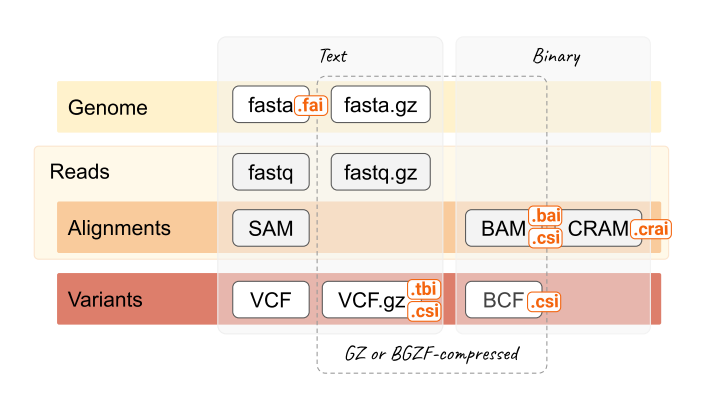
\includegraphics{img/formats_summary.png}
\caption{Data formats summary}
\end{figure}

    \hypertarget{gff}{%
\subsection{GFF}\label{gff}}

One final format worth mentioning is the GFF format. The general feature
format (gene-finding format, generic feature format, GFF) is a file
format used for describing genes and other features of DNA, RNA and
protein sequences. The format consists of one line per feature, each
containing 9 columns of data, seperated by a tab.

Let's look at an example:

\begin{verbatim}
1   Prodigal    CDS 210 1422    .   -   0   ID=s01
1   Prodigal    CDS 508 2464    .   -   0   ID=s02;product=hypothetical protein
1   Prodigal    CDS 967 3525    .   -   0   ID=s03;Name=rfuC;db_xref=COG:COG403
\end{verbatim}

We can see that for each line we have nine fields all seperated by the
tab character:

\begin{enumerate}
\def\labelenumi{\arabic{enumi}.}
\tightlist
\item
  \textbf{seqname} - The name of the sequence where the feature is
  located.
\item
  \textbf{source} - The algorithm or procedure that generated the
  feature. This is typically the name of a software or database.
\item
  \textbf{feature} - The feature type name, like ``gene'', ``exon'' or
  ``cds''.
\item
  \textbf{start} - The start position of the feature, with sequence
  numbering starting at 1.
\item
  \textbf{end} - The end position of the feature, with sequence
  numbering starting at 1.
\item
  \textbf{score} - A numeric value that generally indicates the
  confidence of the source in the annotated feature. A value of ``.'' (a
  dot) is used to define a null value.
\item
  \textbf{strand} - Single character that indicates the strand of the
  feature. This can be ``+'' (positive, or 5'-\textgreater3'), ``-'',
  (negative, or 3'-\textgreater5'), ``.'' (undetermined), or ``?'' for
  features with relevant but unknown strands.
\item
  \textbf{frame} - One of `0', `1' or `2'. `0' indicates that the first
  base of the feature is the first base of a codon, `1' that the second
  base is the first base of a codon, and so on..
\item
  \textbf{attribute} - A semicolon-separated list of tag-value pairs,
  providing additional information about each feature.
\end{enumerate}

    Congratulations you have reached the end of the data formats tutorial!

If you have time then continue to the additional (optional) section of
the tutorial: \href{conversion.ipynb}{Converting between formats}.


    % Add a bibliography block to the postdoc



\newpage





    \hypertarget{converting-between-formats}{%
\section{Converting between formats}\label{converting-between-formats}}

In this section we are going to look at how to convert from one data
format to another. There are many tools available for converting between
formats, and we will use some of the most common ones:
\texttt{samtools}, \texttt{bcftools} and \texttt{Picard}. Although it
might not be obvious yet how this is useful, the tasks are a good way to
become familiar with and understand the different option for the
\texttt{samtools} and \texttt{bcftools}.

\hypertarget{sambam}{%
\subsection{SAM/BAM}\label{sambam}}

To convert between SAM and BAM formats you can use the
\textbf{\texttt{samtools\ view}} command.

To convert a BAM file to a SAM file try:

    \begin{tcolorbox}[breakable, size=fbox, boxrule=1pt, pad at break*=1mm,colback=cellbackground, colframe=cellborder]
\prompt{In}{incolor}{ }{\boxspacing}
\begin{Verbatim}[commandchars=\\\{\}]
samtools\PY{+w}{ }view\PY{+w}{ }\PYZhy{}h\PY{+w}{ }NA20538.bam\PY{+w}{ }\PYZgt{}\PY{+w}{ }NA20538.sam
\end{Verbatim}
\end{tcolorbox}

    Note we use the \textbf{\texttt{-h}} option here to include the header
in the SAM file. Now, have a look at the first five lines of the SAM
file.

    \begin{tcolorbox}[breakable, size=fbox, boxrule=1pt, pad at break*=1mm,colback=cellbackground, colframe=cellborder]
\prompt{In}{incolor}{ }{\boxspacing}
\begin{Verbatim}[commandchars=\\\{\}]
head\PY{+w}{ }\PYZhy{}5\PY{+w}{ }NA20538.sam
\end{Verbatim}
\end{tcolorbox}

    Well that was easy! And converting SAM to BAM is just as
straightforward, try:

    \begin{tcolorbox}[breakable, size=fbox, boxrule=1pt, pad at break*=1mm,colback=cellbackground, colframe=cellborder]
\prompt{In}{incolor}{ }{\boxspacing}
\begin{Verbatim}[commandchars=\\\{\}]
samtools\PY{+w}{ }view\PY{+w}{ }\PYZhy{}b\PY{+w}{ }NA20538.sam\PY{+w}{ }\PYZgt{}\PY{+w}{ }NA20538\PYZus{}2.bam
\end{Verbatim}
\end{tcolorbox}

    This time there is no need for the \textbf{\texttt{-h}} option, however
we have to tell \texttt{samtools} that we want the output in BAM format.
We do this by adding the \textbf{\texttt{-b}} option. Note we have
called the file \texttt{NA20538\_2.bam} so that the original
\texttt{NA20538.bam} file is not overwritten.

Check the conversion was successful.

First check the header section:

    \begin{tcolorbox}[breakable, size=fbox, boxrule=1pt, pad at break*=1mm,colback=cellbackground, colframe=cellborder]
\prompt{In}{incolor}{ }{\boxspacing}
\begin{Verbatim}[commandchars=\\\{\}]
samtools\PY{+w}{ }view\PY{+w}{ }\PYZhy{}h\PY{+w}{ }NA20538\PYZus{}2.bam\PY{+w}{ }\PY{p}{|}\PY{+w}{ }head\PY{+w}{ }\PYZhy{}5
\end{Verbatim}
\end{tcolorbox}

    Then check the alignment section:

    \begin{tcolorbox}[breakable, size=fbox, boxrule=1pt, pad at break*=1mm,colback=cellbackground, colframe=cellborder]
\prompt{In}{incolor}{ }{\boxspacing}
\begin{Verbatim}[commandchars=\\\{\}]
samtools\PY{+w}{ }view\PY{+w}{ }NA20538\PYZus{}2.bam\PY{+w}{ }\PY{p}{|}\PY{+w}{ }head\PY{+w}{ }\PYZhy{}5
\end{Verbatim}
\end{tcolorbox}

    \hypertarget{bamcram}{%
\subsection{BAM/CRAM}\label{bamcram}}

The \textbf{\texttt{samtools\ view}} command can also be used to convert
betwen BAM and CRAM formats. In the data directory there is a BAM file
called \texttt{yeast.bam} that was created by aligning \textit{S.
cerevisiae} Illumina data to the reference genome
\texttt{Saccharomyces\_cerevisiae.EF4.68.dna.toplevel.fa}.

To convert a BAM to a CRAM, try

    \begin{tcolorbox}[breakable, size=fbox, boxrule=1pt, pad at break*=1mm,colback=cellbackground, colframe=cellborder]
\prompt{In}{incolor}{ }{\boxspacing}
\begin{Verbatim}[commandchars=\\\{\}]
samtools\PY{+w}{ }view\PY{+w}{ }\PYZhy{}C\PY{+w}{ }\PYZhy{}T\PY{+w}{ }Saccharomyces\PYZus{}cerevisiae.EF4.68.dna.toplevel.fa\PY{+w}{ }\PY{l+s+se}{\PYZbs{}}
\PYZhy{}o\PY{+w}{ }yeast.cram\PY{+w}{ }yeast.bam
\end{Verbatim}
\end{tcolorbox}

    Here, we use the \textbf{\texttt{-C}} option to tell \texttt{samtools}
we want the output as CRAM, and the \textbf{\texttt{-T}} option to
specify what reference file to use for the conversion. We also use the
\textbf{\texttt{-o}} option to specify the name of the output file.

    Have a look at what files were created:

    \begin{tcolorbox}[breakable, size=fbox, boxrule=1pt, pad at break*=1mm,colback=cellbackground, colframe=cellborder]
\prompt{In}{incolor}{ }{\boxspacing}
\begin{Verbatim}[commandchars=\\\{\}]
ls\PY{+w}{ }\PYZhy{}l
\end{Verbatim}
\end{tcolorbox}

    As you can see, this has created an index file for the reference genome
called \texttt{Saccharomyces\_cerevisiae.EF4.68.dna.toplevel.fa.fai} and
the CRAM file \texttt{yeast.cram}.

    Check the conversion was successful:

    \begin{tcolorbox}[breakable, size=fbox, boxrule=1pt, pad at break*=1mm,colback=cellbackground, colframe=cellborder]
\prompt{In}{incolor}{ }{\boxspacing}
\begin{Verbatim}[commandchars=\\\{\}]
samtools\PY{+w}{ }view\PY{+w}{ }yeast.cram\PY{+w}{ }\PY{p}{|}\PY{+w}{ }head\PY{+w}{ }\PYZhy{}5
\end{Verbatim}
\end{tcolorbox}

    \hypertarget{exercises}{%
\subsubsection{Exercises}\label{exercises}}

\textbf{Q1: Since CRAM files use reference-based compression, we expect
the CRAM file to be smaller than the BAM file. What is the size of the
CRAM file?}

    \begin{tcolorbox}[breakable, size=fbox, boxrule=1pt, pad at break*=1mm,colback=cellbackground, colframe=cellborder]
\prompt{In}{incolor}{ }{\boxspacing}
\begin{Verbatim}[commandchars=\\\{\}]

\end{Verbatim}
\end{tcolorbox}

    \textbf{Q2: Why do we need to provide the reference genome when
converting to CRAM format?}

    \begin{tcolorbox}[breakable, size=fbox, boxrule=1pt, pad at break*=1mm,colback=cellbackground, colframe=cellborder]
\prompt{In}{incolor}{ }{\boxspacing}
\begin{Verbatim}[commandchars=\\\{\}]

\end{Verbatim}
\end{tcolorbox}

    \textbf{Q3: Convert the CRAM file back to a BAM file called
yeast\_2.bam?}

    \begin{tcolorbox}[breakable, size=fbox, boxrule=1pt, pad at break*=1mm,colback=cellbackground, colframe=cellborder]
\prompt{In}{incolor}{ }{\boxspacing}
\begin{Verbatim}[commandchars=\\\{\}]

\end{Verbatim}
\end{tcolorbox}

    \hypertarget{fastq-to-sambamcram}{%
\subsection{FASTQ to SAM/BAM/CRAM}\label{fastq-to-sambamcram}}

SAM format is mainly used to store alignment data, however in some cases
we may want to store the unaligned data in SAM format and for this we
can use the picard tools \textbf{\texttt{FastqToSam}} application.
\href{https://broadinstitute.github.io/picard/}{Picard tools} is a Java
application with a number of useful options for manipulating sequence
data.

To convert the FASTQ files from sequencing run 13681\_1\_18 to unaligned
SAM format, try:

    \begin{tcolorbox}[breakable, size=fbox, boxrule=1pt, pad at break*=1mm,colback=cellbackground, colframe=cellborder]
\prompt{In}{incolor}{ }{\boxspacing}
\begin{Verbatim}[commandchars=\\\{\}]
picard\PY{+w}{ }FastqToSam\PY{+w}{ }\PY{n+nv}{F1}\PY{o}{=}13681\PYZus{}1\PYZus{}18\PYZus{}1.fastq.gz\PY{+w}{ }\PY{n+nv}{F2}\PY{o}{=}13681\PYZus{}1\PYZus{}18\PYZus{}2.fastq.gz\PY{+w}{ }\PY{l+s+se}{\PYZbs{}}
\PY{n+nv}{O}\PY{o}{=}13681\PYZus{}1\PYZus{}18.sam\PY{+w}{ }\PY{n+nv}{SM}\PY{o}{=}13681\PYZus{}1\PYZus{}18
\end{Verbatim}
\end{tcolorbox}

    Here, the \textbf{\texttt{F1}} and \textbf{\texttt{F2}} options are the
paired end FASTQ files, the \textbf{\texttt{O}} option is used to
specify the name of the output SAM file and \textbf{\texttt{SM}} is the
sample name which will be stored in the header of the SAM file. There
are also multiple other options for specifying what metadata to include
in the SAM header. To see all available options, run:

    \begin{tcolorbox}[breakable, size=fbox, boxrule=1pt, pad at break*=1mm,colback=cellbackground, colframe=cellborder]
\prompt{In}{incolor}{ }{\boxspacing}
\begin{Verbatim}[commandchars=\\\{\}]
picard\PY{+w}{ }FastqToSam\PY{+w}{ }\PYZhy{}h
\end{Verbatim}
\end{tcolorbox}

    Check the conversion was successful:

    \begin{tcolorbox}[breakable, size=fbox, boxrule=1pt, pad at break*=1mm,colback=cellbackground, colframe=cellborder]
\prompt{In}{incolor}{ }{\boxspacing}
\begin{Verbatim}[commandchars=\\\{\}]
head\PY{+w}{ }\PYZhy{}5\PY{+w}{ }13681\PYZus{}1\PYZus{}18.sam
\end{Verbatim}
\end{tcolorbox}

    From here you can convert the SAM file to BAM and CRAM, as described
previously.

    \hypertarget{cram-to-fastq}{%
\subsection{CRAM to FASTQ}\label{cram-to-fastq}}

The \textbf{\texttt{samtools\ fastq}} command can be used to convert
CRAM to FASTQ directly. However, for many applications we need the FASTQ
files ordered so that the order of the reads in the first file match the
order of the reads in the second file. This is to allow the reads in a
fragment to be matched up based on their location in the FASTQ file. For
this reason, we first use \textbf{\texttt{samtools\ collate}} to produce
a collated BAM file which ensures that reads of the same name (and
therefore from the same fragment) are grouped together in contiguous
groups.

    \begin{tcolorbox}[breakable, size=fbox, boxrule=1pt, pad at break*=1mm,colback=cellbackground, colframe=cellborder]
\prompt{In}{incolor}{ }{\boxspacing}
\begin{Verbatim}[commandchars=\\\{\}]
samtools\PY{+w}{ }collate\PY{+w}{ }yeast.cram\PY{+w}{ }yeast.collated
\end{Verbatim}
\end{tcolorbox}

    Have a look at what files were created:

    \begin{tcolorbox}[breakable, size=fbox, boxrule=1pt, pad at break*=1mm,colback=cellbackground, colframe=cellborder]
\prompt{In}{incolor}{ }{\boxspacing}
\begin{Verbatim}[commandchars=\\\{\}]
ls
\end{Verbatim}
\end{tcolorbox}

    The newly produced BAM file will be called \texttt{yeast.collated.bam}.
Have a look at the contents and notice how the order of the reads
differs from the \texttt{yeast.cram} file:

    \begin{tcolorbox}[breakable, size=fbox, boxrule=1pt, pad at break*=1mm,colback=cellbackground, colframe=cellborder]
\prompt{In}{incolor}{ }{\boxspacing}
\begin{Verbatim}[commandchars=\\\{\}]
samtools\PY{+w}{ }view\PY{+w}{ }yeast.collated.bam\PY{+w}{ }\PY{p}{|}\PY{+w}{ }head\PY{+w}{ }\PYZhy{}6
\end{Verbatim}
\end{tcolorbox}

    Let's use this to create two FASTQ files, one for the first reads of the
fragment and one for the second reads of the fragment:

    \begin{tcolorbox}[breakable, size=fbox, boxrule=1pt, pad at break*=1mm,colback=cellbackground, colframe=cellborder]
\prompt{In}{incolor}{ }{\boxspacing}
\begin{Verbatim}[commandchars=\\\{\}]
samtools\PY{+w}{ }fastq\PY{+w}{ }\PYZhy{}N\PY{+w}{ }\PYZhy{}1\PY{+w}{ }yeast.collated\PYZus{}1.fastq\PY{+w}{ }\PYZhy{}2\PY{+w}{ }yeast.collated\PYZus{}2.fastq\PY{+w}{ }\PY{l+s+se}{\PYZbs{}}
yeast.collated.bam
\end{Verbatim}
\end{tcolorbox}

    Here, we use the \textbf{\texttt{-N}} option to tell \texttt{samtools}
to include the /1 and /2 in the read name.

Check the conversion was succesful:

    \begin{tcolorbox}[breakable, size=fbox, boxrule=1pt, pad at break*=1mm,colback=cellbackground, colframe=cellborder]
\prompt{In}{incolor}{ }{\boxspacing}
\begin{Verbatim}[commandchars=\\\{\}]
head\PY{+w}{ }\PYZhy{}4\PY{+w}{ }yeast.collated\PYZus{}1.fastq
head\PY{+w}{ }\PYZhy{}4\PY{+w}{ }yeast.collated\PYZus{}2.fastq
\end{Verbatim}
\end{tcolorbox}

    \hypertarget{vcfbcf}{%
\subsection{VCF/BCF}\label{vcfbcf}}

In a similar way that \textbf{\texttt{samtools\ view}} can be used to
convert between SAM, BAM and CRAM, \textbf{\texttt{bcftools\ view}} can
be used to convert between VCF and BCF.

To convert a BCF file to a VCF file try:

    \begin{tcolorbox}[breakable, size=fbox, boxrule=1pt, pad at break*=1mm,colback=cellbackground, colframe=cellborder]
\prompt{In}{incolor}{ }{\boxspacing}
\begin{Verbatim}[commandchars=\\\{\}]
bcftools\PY{+w}{ }view\PY{+w}{ }\PYZhy{}O\PY{+w}{ }v\PY{+w}{ }\PYZhy{}o\PY{+w}{ }1kg.vcf\PY{+w}{ }1kg.bcf
\end{Verbatim}
\end{tcolorbox}

    The \textbf{\texttt{-O}} option allows us to specify in what format we
want the output, compressed BCF (b), uncompressed BCF (u), compressed
VCF (z) or uncompressed VCF (v). With the \textbf{\texttt{-o}} option we
can select the name of the output file.

Have a look at what files were generated (the options \texttt{-lrt} will
list the files in reverse chronological order):

    \begin{tcolorbox}[breakable, size=fbox, boxrule=1pt, pad at break*=1mm,colback=cellbackground, colframe=cellborder]
\prompt{In}{incolor}{ }{\boxspacing}
\begin{Verbatim}[commandchars=\\\{\}]
ls\PY{+w}{ }\PYZhy{}lrt
\end{Verbatim}
\end{tcolorbox}

    Check the conversion was successful:

    \begin{tcolorbox}[breakable, size=fbox, boxrule=1pt, pad at break*=1mm,colback=cellbackground, colframe=cellborder]
\prompt{In}{incolor}{ }{\boxspacing}
\begin{Verbatim}[commandchars=\\\{\}]
bcftools\PY{+w}{ }view\PY{+w}{ }1kg.vcf\PY{+w}{ }\PY{p}{|}\PY{+w}{ }head\PY{+w}{ }\PYZhy{}10
\end{Verbatim}
\end{tcolorbox}

    To convert a VCF file to BCF, try:

    \begin{tcolorbox}[breakable, size=fbox, boxrule=1pt, pad at break*=1mm,colback=cellbackground, colframe=cellborder]
\prompt{In}{incolor}{ }{\boxspacing}
\begin{Verbatim}[commandchars=\\\{\}]
bcftools\PY{+w}{ }view\PY{+w}{ }\PYZhy{}O\PY{+w}{ }b\PY{+w}{ }\PYZhy{}o\PY{+w}{ }1kg\PYZus{}2.bcf\PY{+w}{ }1kg.vcf
\end{Verbatim}
\end{tcolorbox}

    Note we have called the file \texttt{1kg\_2.bcf} so that the original
\texttt{1kg.bcf} file is not overwritten.

    Check the conversion was successful:

    \begin{tcolorbox}[breakable, size=fbox, boxrule=1pt, pad at break*=1mm,colback=cellbackground, colframe=cellborder]
\prompt{In}{incolor}{ }{\boxspacing}
\begin{Verbatim}[commandchars=\\\{\}]
bcftools\PY{+w}{ }view\PY{+w}{ }1kg\PYZus{}2.bcf\PY{+w}{ }\PY{p}{|}\PY{+w}{ }head\PY{+w}{ }\PYZhy{}10
\end{Verbatim}
\end{tcolorbox}

    \hypertarget{exercises}{%
\subsubsection{Exercises}\label{exercises}}

\textbf{Q4: Convert the BCF file 1kg.bcf to a compressed VCF file called
1kg.vcf.gz}

    \begin{tcolorbox}[breakable, size=fbox, boxrule=1pt, pad at break*=1mm,colback=cellbackground, colframe=cellborder]
\prompt{In}{incolor}{ }{\boxspacing}
\begin{Verbatim}[commandchars=\\\{\}]

\end{Verbatim}
\end{tcolorbox}

    \textbf{Congratulations} you have reached the end of the tutorial!


    % Add a bibliography block to the postdoc



\end{document}
